%!TEX root = ../template.tex
%%%%%%%%%%%%%%%%%%%%%%%%%%%%%%%%%%%%%%%%%%%%%%%%%%%%%%%%%%%%%%%%%%%
%% chapter4.tex
%% NOVA thesis document file
%%
%% Chapter 4: Technological Implementation
%%%%%%%%%%%%%%%%%%%%%%%%%%%%%%%%%%%%%%%%%%%%%%%%%%%%%%%%%%%%%%%%%%%

\typeout{NT FILE chapter4.tex}%

\chapter{Technological Implementation}
\label{cha:implementation}

This chapter describes how the \gls{DT} framework from \Cref{cha:architecture} was built in practice, covering the tools, protocols, and software components used at each layer. Moving from high-level architectural specifications to an operational system requires bridging the gap between abstract standards, such as the \gls{AAS}, and the practical realities of industrial hardware and game-engine physics.

A fourth step, Layer~0, is also introduced here. While the conceptual architecture assumes 3D geometric models are readily available, the physical \gls{FMS} testbed used in this work lacked pre-existing \gls{CAD} assets. Layer~0 addresses this gap by establishing a manual digitization workflow in Blender, producing the lightweight 3D models required before the configuration pipeline can begin.

\section{System Architecture and Technology Realization}
\label{sec:tech_realization}

\subsection{Physical Testbed Context: The Modular FMS Bench}
To validate the framework under real-world conditions, an existing \gls{FMS} testbed was used as the pilot case study (\Cref{fig:fms_pilot_testbed}), based on the modular \gls{CPPS} architecture proposed by \textcite{Rocha2024}. The setup is a modular closed-loop conveyor system used for product transportation across processing and inspection stations. Using a modular testbed provides an ideal scenario to test whether the proposed \gls{DT} can reconstruct a factory floor modularly, asset by asset, and coordinate multiple distributed mechanisms in real time.

\begin{figure}[htbp]
    \centering
    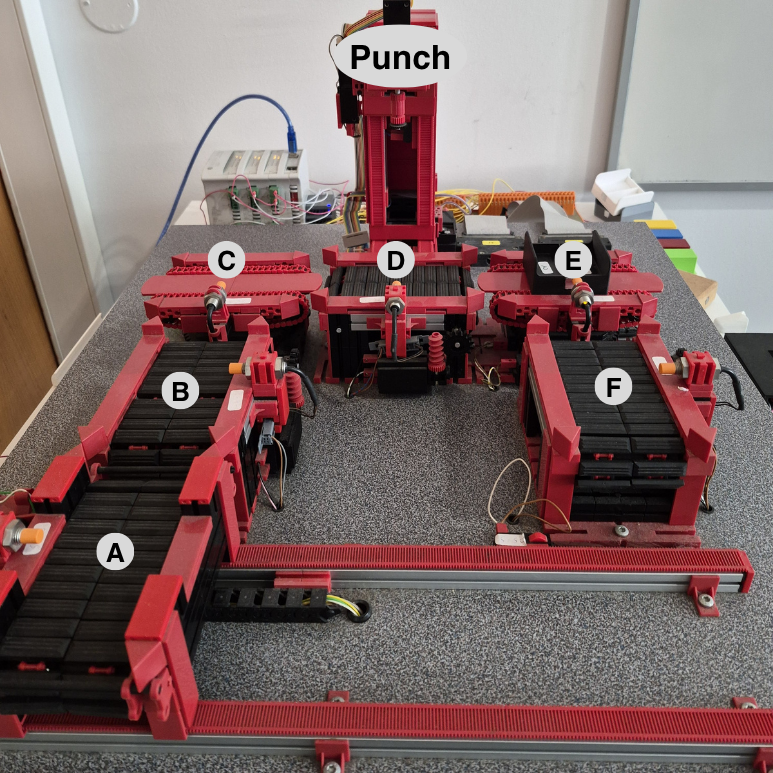
\includegraphics[width=0.72\linewidth,height=0.42\textheight,keepaspectratio]{5-Figures/fms_pilot_bench.jpg}
    \caption{Physical modular \gls{FMS} conveyor testbed used as the validation environment, showing the modular conveyor tracks, magnetic sensors, the punch system, and the Industrial Shields M-DUINO \gls{PLC} controller.}
    \label{fig:fms_pilot_testbed}
\end{figure}

Mechanically, the physical bench comprises three stationary conveyor belts (Conveyor B, Conveyor D, and Conveyor F), two rotational conveyor sections (Conveyor C and Conveyor E), one translating transfer conveyor (Conveyor A), and a vertical punch mechanism that simulates drilling, stamping, or screwing operations on the product. Field instrumentation includes 24\,V~DC magnetic sensors distributed along the tracks for product detection, contact limit switches for tracking conveyor and punch positions, and 24\,V~DC motors driving each section. Control is handled by an Industrial Shields M-DUINO 57R+ \gls{PLC} (built around the Arduino Mega 2560 architecture), equipped with an integrated Ethernet interface and optoisolated \gls{IO} terminal boards. The controller maps field devices across indexed \gls{IO} registers: digital input pins (I0\_0 to I2\_3) capture sensor states, while relay output pins (R0\_2 to R2\_8) command conveyor movement, and punch actions (the complete hardware pin assignment is detailed in \Cref{app:fms_io_mapping}).

\subsection{Overall Component Architecture and Inter-Layer Interfaces}
With this physical bench as the target, the complete framework was implemented across four operational layers. \Cref{fig:architecture_global} illustrates the system implementation as a component diagram.

\begin{figure}[htbp]
    \centering
    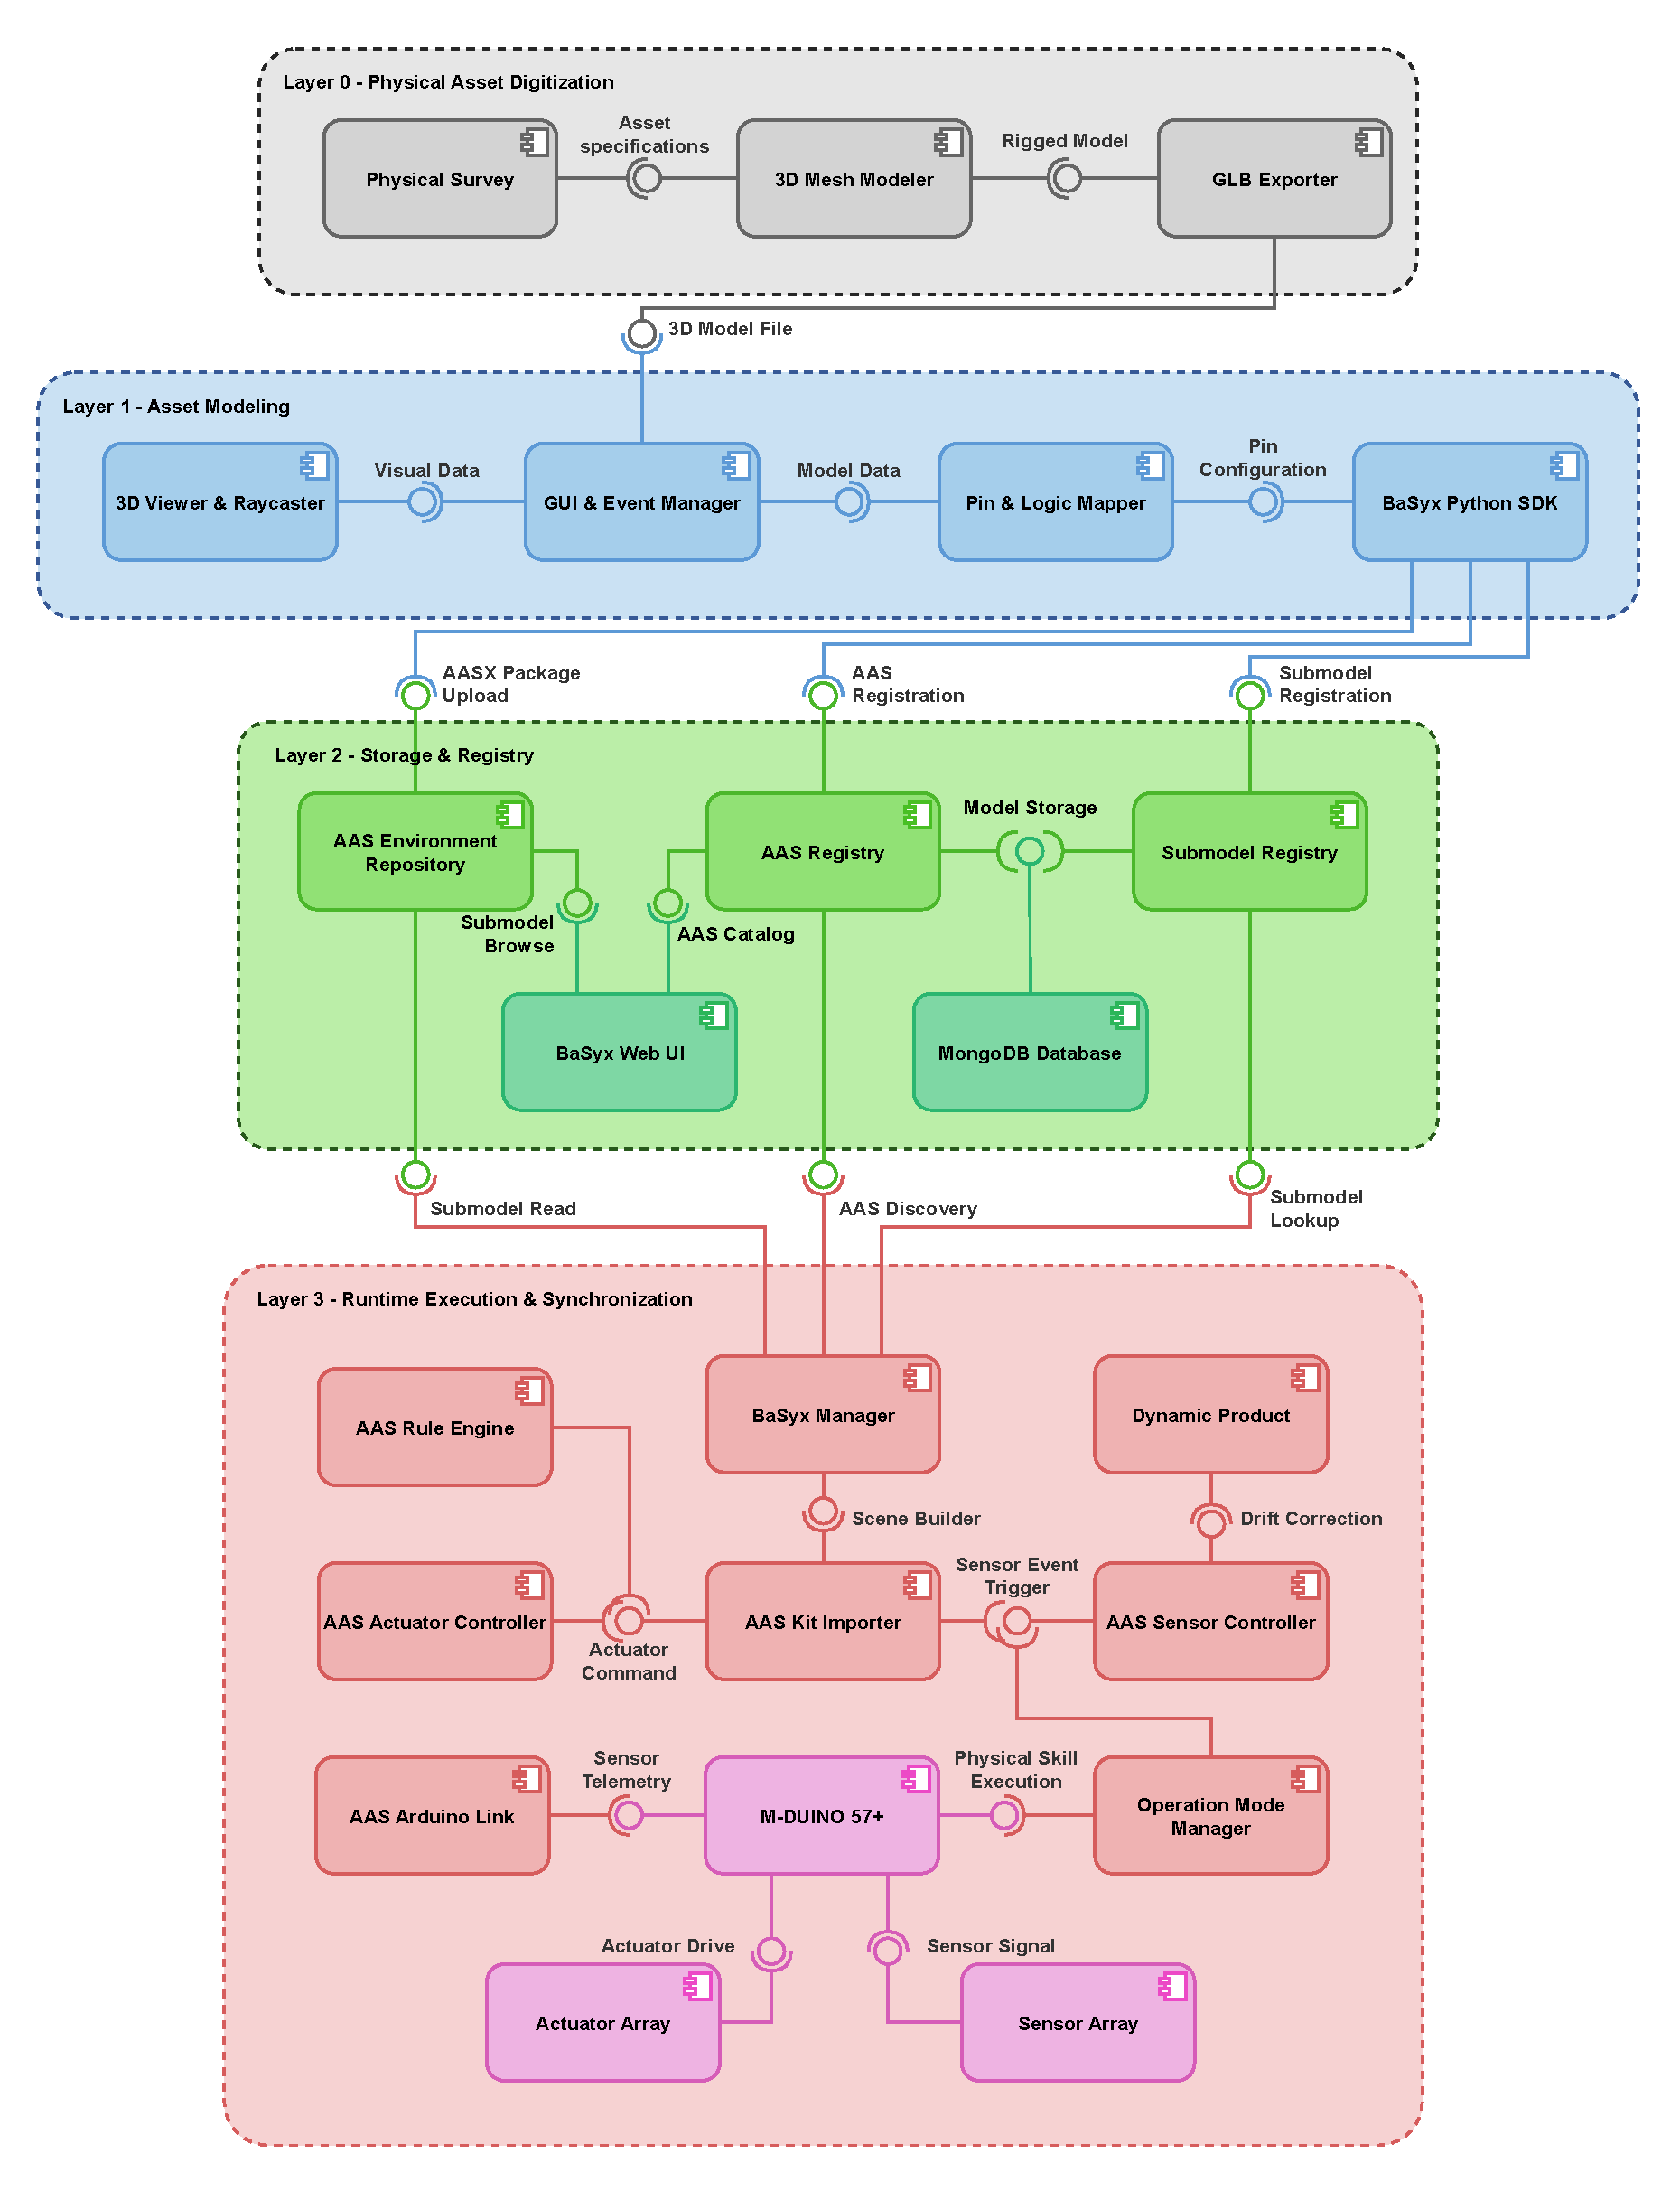
\includegraphics[width=\textwidth]{5-Figures/Implementação.drawio.pdf}
    \caption[Implementation architecture of the framework]{Implementation architecture of the framework: (0) Physical Asset Digitization in Blender, (1) Asset Modeling in the Python desktop application, (2) Storage and Registry in Eclipse BaSyx~v2 on Docker, and (3) Runtime Execution and Physical Synchronization in Unity 3D with an Industrial Shields M-DUINO \gls{PLC}.}
    \label{fig:architecture_global}
\end{figure}

The information flow spans four operational stages. In Layer~0 (Physical Asset Digitization), physical hardware components are rebuilt as 3D models in Blender using manual measurements with a tape measure. These parts are rigged with appropriate pivot origins and sensor triggers and then exported as binary \gls{glTF} files. Next, Layer~1 (Asset Modeling) runs within a custom interactive desktop asset creation tool, loading the 3D model into an interactive viewport. Here, users configure machine properties and assign \gls{IO} pins before the BaSyx Python \gls{SDK} packages everything into an AASX bundle and uploads it to Layer~2 through \gls{REST} endpoints. 

In Layer~2 (Storage and Registry), Eclipse BaSyx~v2 services run inside Docker containers. An \gls{AAS} Environment Repository stores package files, while the \gls{AAS} Registry and Submodel Registry track active assets and submodel endpoints backed by MongoDB. Operators can inspect these assets through the BaSyx Web \gls{GUI} using browsing endpoints. Finally, Layer~3 (Runtime Execution and Physical Synchronization) executes the 3D simulation in Unity, connecting it directly to the physical testbed controlled by the Industrial Shields M-DUINO \gls{PLC}. At launch, Unity queries BaSyx to retrieve models and procedurally assemble the scene. During operation, the runtime either performs \gls{VC} through local logic rules or executes live physical synchronization by exchanging low-latency \gls{TCP} telemetry and \gls{HTTP} skill executions tied directly to the field sensors and actuator drives.

\section{Layer 0: Physical Asset Digitization and 3D Modeling (Blender)}
\label{sec:impl_layer0}

In existing industrial automation setups, physical equipment often has no digital 3D counterpart. Where original \gls{CAD} drawings do exist, they tend to include excessive geometric detail, like thread profiles and internal fasteners, that is too complex for real-time simulation. At the same time, they usually lack the joint hierarchies and pivot definitions that a physics engine needs to animate moving parts.

The \gls{FMS} testbed in this work had no usable 3D models at all. A manual digitization phase was carried out in Blender 5.2.0 LTS to produce the assets from scratch. This phase is called Layer~0 because it happens before the software pipeline starts, and its output, a set of GLB files, is what the rest of the system depends on.

\Cref{fig:component_layer0} shows the component structure of Layer~0, which divides into three sequential tasks. First, the Physical Survey uses a tape measure on the physical \gls{FMS} bench to measure parts accurately, providing the asset specifications needed for \gls{CAD} reconstruction. Next, the 3D Mesh Modeler uses these measurements to build clean low-poly parts, aligning rotation pivots for moving components to produce a validated rigged model. Finally, the GLB Exporter packages the 3D geometry, hierarchy, and materials into a single binary file ready for Layer~1.

\begin{figure}[htbp]
    \centering
    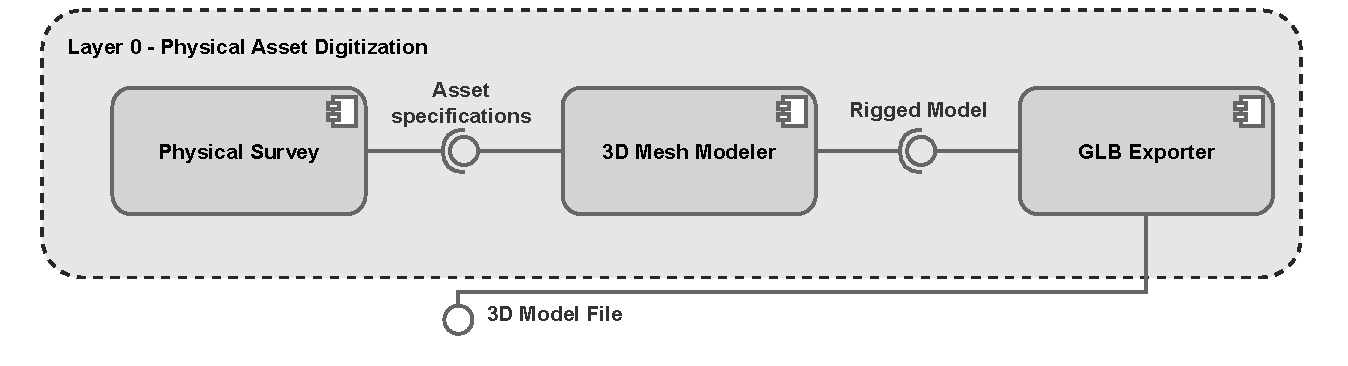
\includegraphics[width=\linewidth,height=0.72\textheight,keepaspectratio]{5-Figures/Layer 0 - Physical Asset Digitization.pdf}
    \caption{Component architecture and interface boundaries of Layer 0 (Physical Asset Digitization).}
    \label{fig:component_layer0}
\end{figure}

\subsection{Dimensional Survey and Polygonal Reconstruction}
Manual measurements were taken across the physical \gls{FMS} conveyor bench. Each module was reconstructed to 1:1 scale, matching Unity's coordinate system. The polygonal geometry was modeled with a low-poly approach for real-time simulation: contact and visual surfaces were kept precise to ensure correct physical interactions with moving products, while non-functional internal cavities, hidden screws, and fasteners were omitted to reduce polygon count and memory footprint.

\begin{figure}[htbp]
    \centering
    \begin{subfigure}[t]{0.48\textwidth}
        \centering
        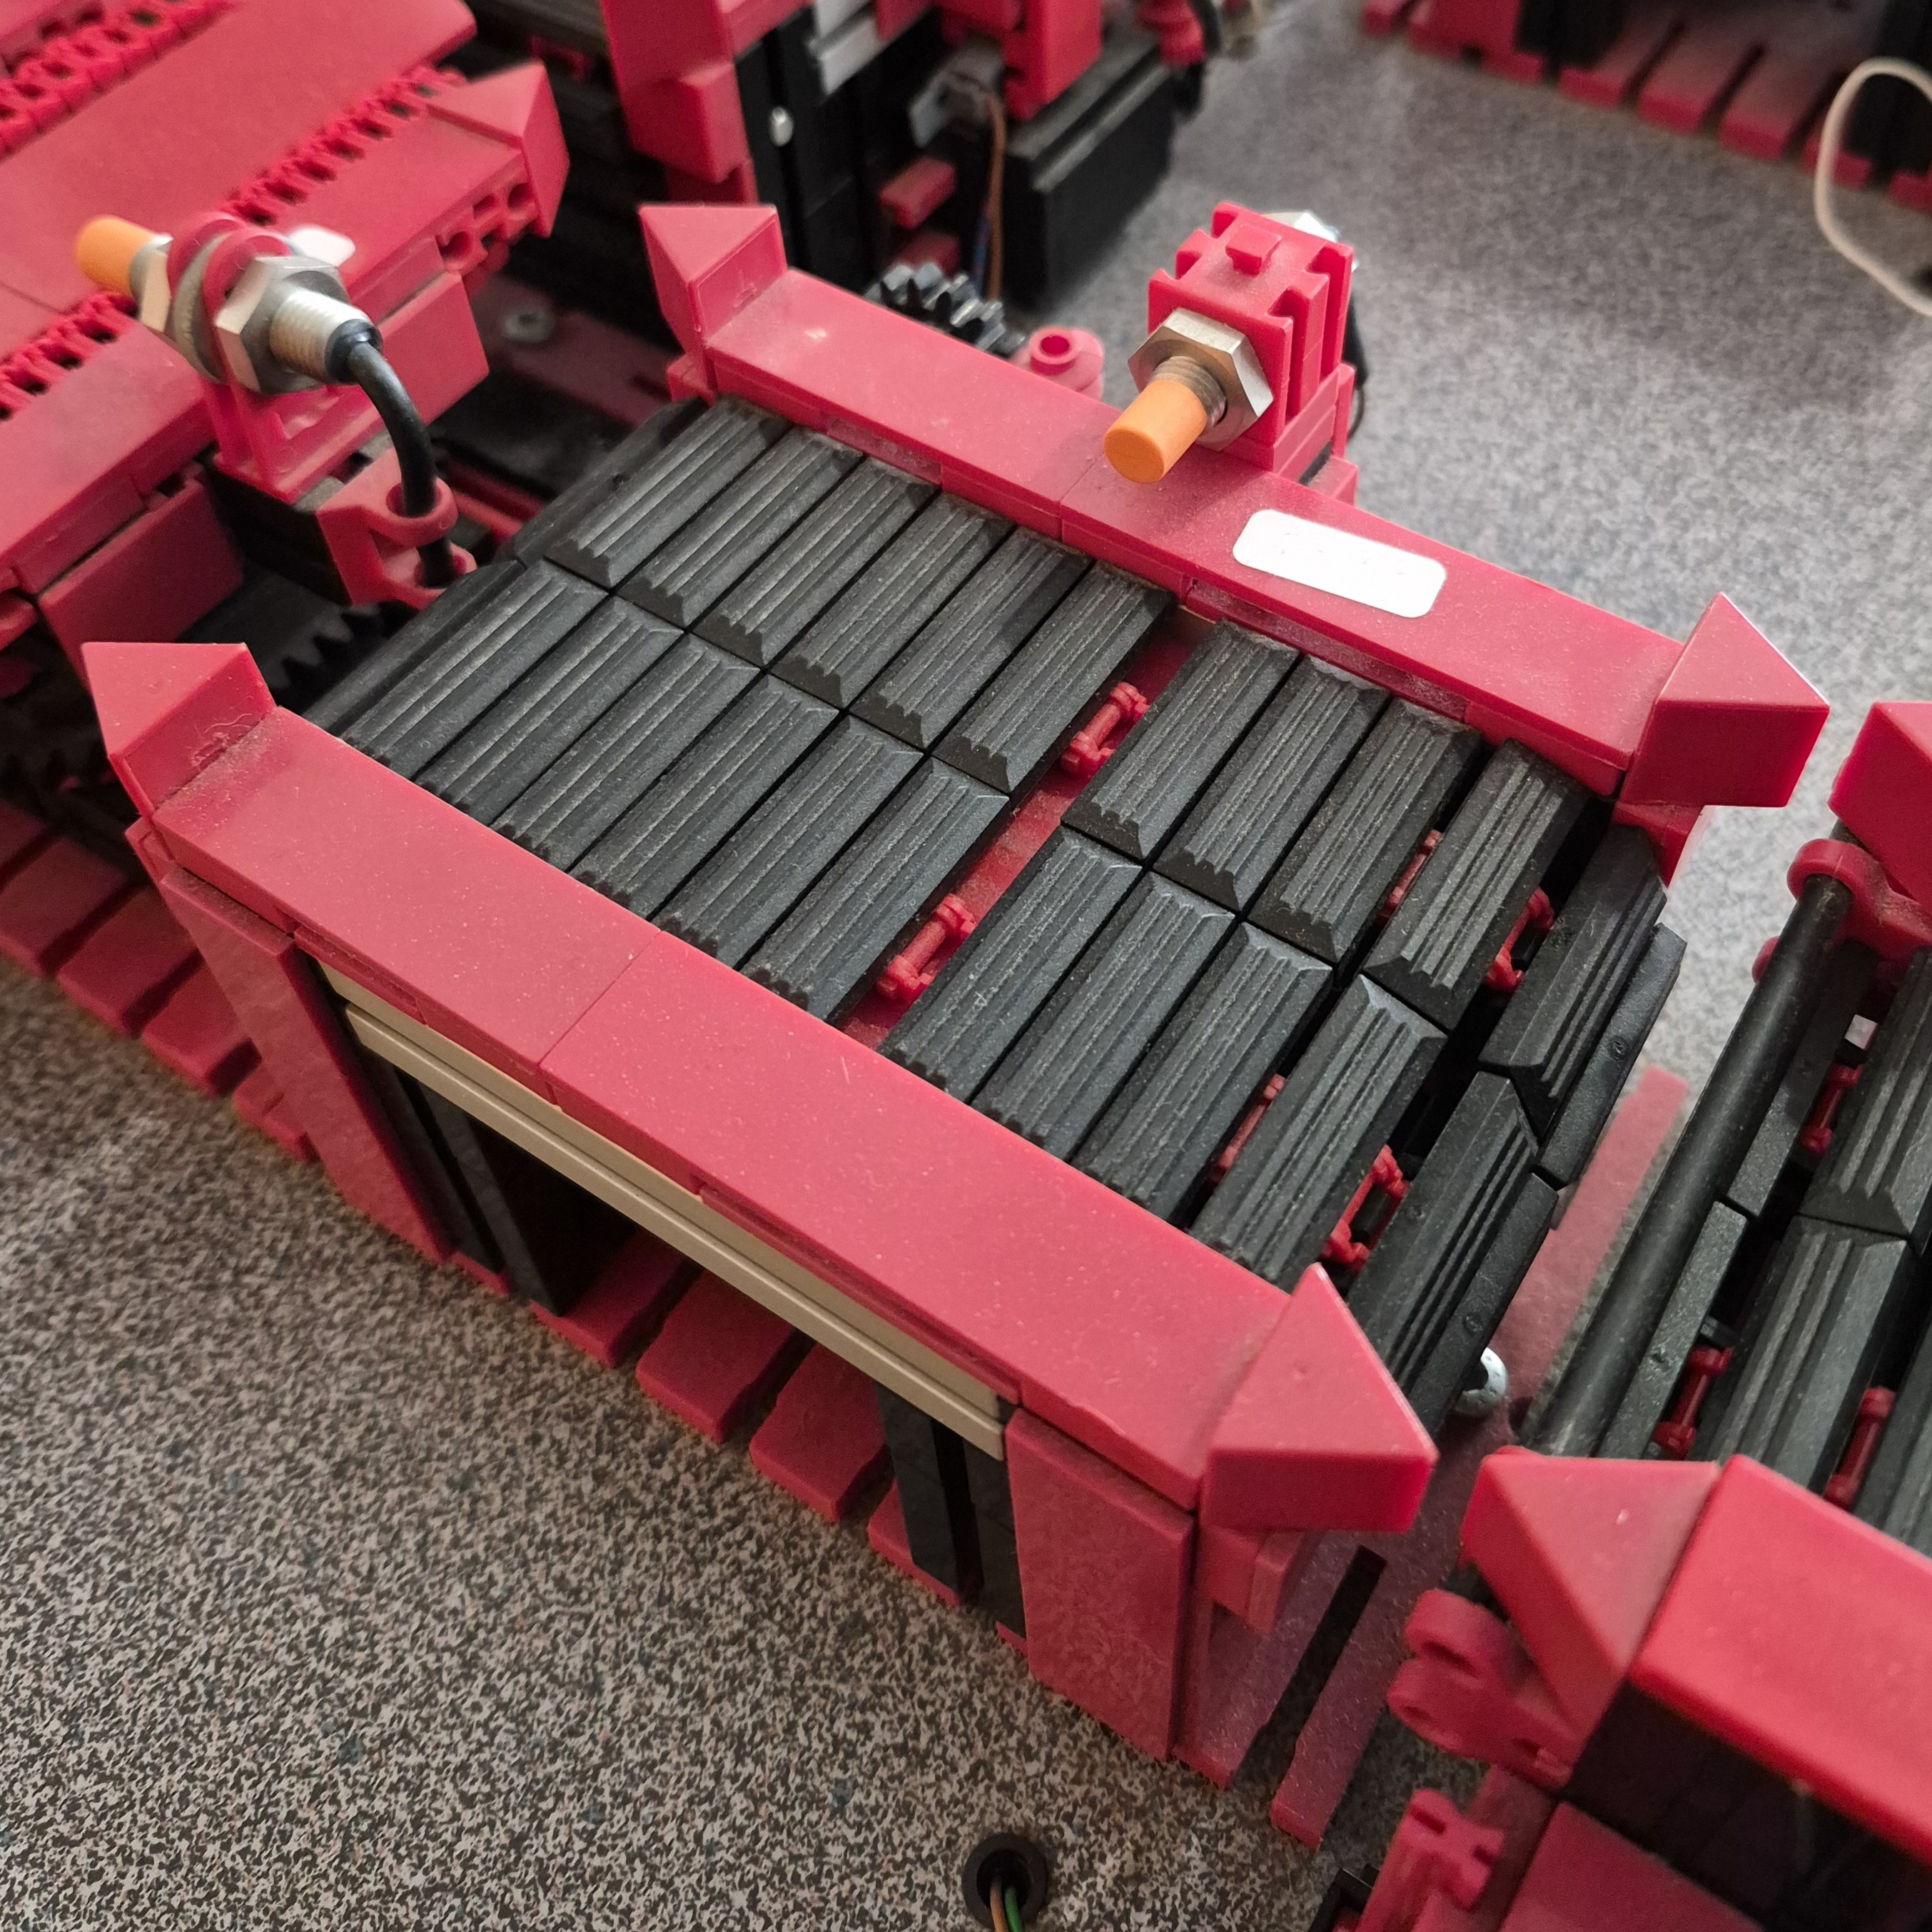
\includegraphics[width=\linewidth,height=5.8cm,keepaspectratio]{5-Figures/fms_conveyor_sensors_closeup.jpg}
        \caption{Physical conveyor module.}
        \label{fig:fms_physical_module}
    \end{subfigure}
    \hfill
    \begin{subfigure}[t]{0.48\textwidth}
        \centering
        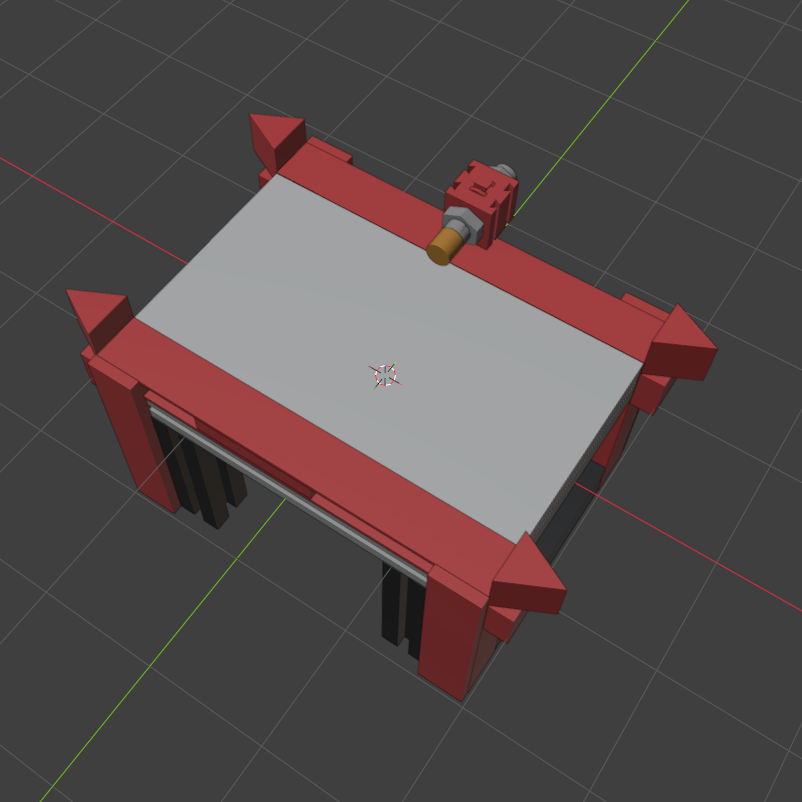
\includegraphics[width=\linewidth,height=5.8cm,keepaspectratio]{5-Figures/blender_kLfhitpziL.png}
        \caption{Reconstructed 3D asset.}
        \label{fig:blender_3d_module}
    \end{subfigure}
    \caption{Comparison between the physical modular \gls{FMS} conveyor module and its reconstructed 3D simulation model in Blender.}
    \label{fig:fms_physical_vs_blender}
\end{figure}

\subsection{Kinematic Hierarchy and Origin Alignment}
To satisfy the requirements of the \textit{VisualStructure} model (\Cref{sec:model_visual_structure}), each asset was structured into an explicit parent-child hierarchy separating static frames from movable components. Static frames were joined into a single root node with its coordinate origin set at the base reference point $(0, 0, 0)$. Movable elements, such as belts, were isolated into child objects. Crucially, the origin (pivot) of each moving mesh was aligned precisely with its physical axis of rotation or linear motion vector. Accurate pivot placement is vital because any offset causes the component to wobble or rotate around the wrong axis when driven by \textit{BehaviorBinding} in the runtime engine (\Cref{sec:model_behavior_mapping}). Where required, invisible sensor trigger volumes were also integrated into the model geometry to detect the passage of dynamic products during simulation.

\subsection{Asset Export and Interchange Formats}
Once assembled, the 3D models were exported using the open \gls{glTF}/GLB standard. GLB packs polygonal meshes, transform node hierarchies, materials, and textures into one binary file, which is the format the Asset Modeling layer reads.

\section{Layer 1: Asset Modeling Desktop Application}
\label{sec:impl_wizard}

The Layer~1 implementation was realized as a standalone desktop application. It merges the Asset Model Editor and Package Exporter roles from \Cref{sec:layer1_conceptual} into a single graphical environment. The goal, in line with requirement \textbf{NFR4}, was to let engineers configure a \gls{DT} asset without needing to write any code.

\Cref{fig:component_layer1} shows the component structure of the desktop application suite, split into four collaborating modules. The 3D Viewer \& Raycaster embeds an interactive viewport to display the asset. The \gls{GUI} \& Event Manager provides the PyQt6 interface that leads the user through configuration tabs and consolidates settings into structured model data. The Pin \& Logic Mapper maps these visual sensor locations directly to physical controller pins. Finally, the BaSyx Python \gls{SDK} generates the corresponding \gls{AAS} submodels in memory, packages the complete AASX archive, and registers it with Layer~2 through dedicated \gls{REST} endpoints for package upload, shell registration, and submodel registration.

\begin{figure}[htbp]
    \centering
    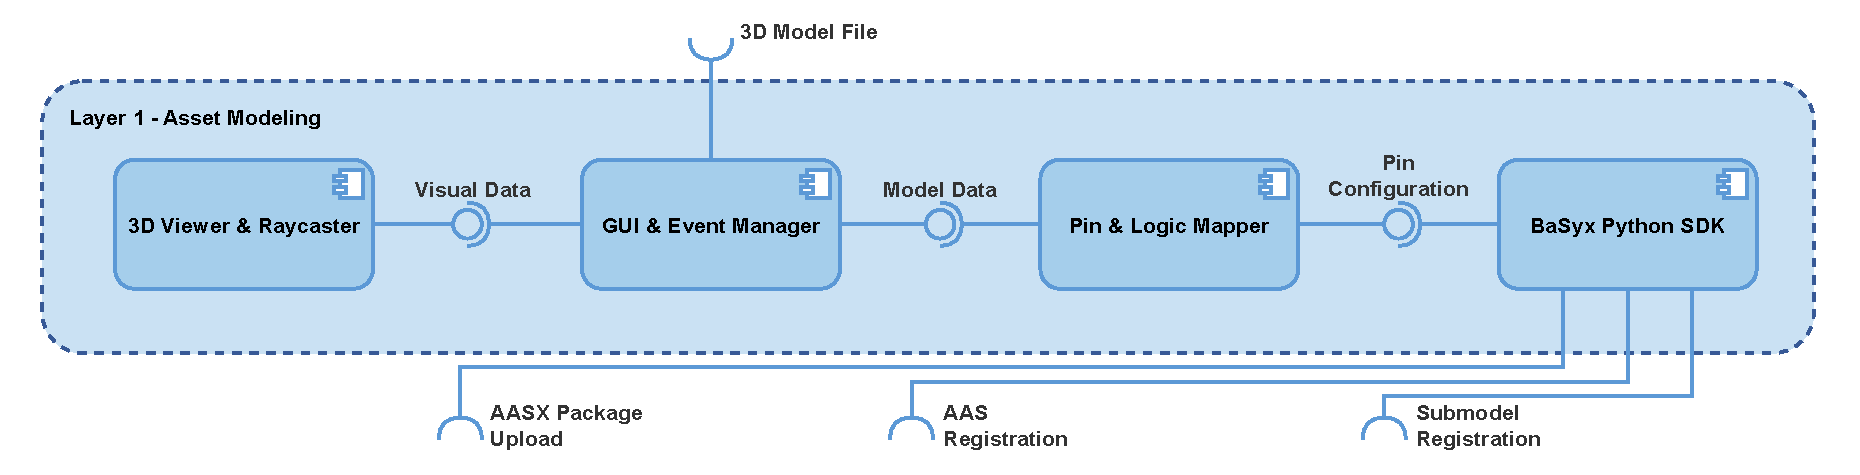
\includegraphics[width=\linewidth,height=0.72\textheight,keepaspectratio]{5-Figures/Layer 1 - Asset Modeling.pdf}
    \caption{Component architecture and interface boundaries of Layer 1 (Asset Modeling).}
    \label{fig:component_layer1}
\end{figure}

\subsection{\texorpdfstring{\gls{AAS}}{AAS} Data Model \& Submodel Specifications}
Rather than forcing a rigid linear sequence, the modeling tool acts as a semantic editor that populates standardized IEC~63278 \gls{AAS} submodels, as conceptualized in \Cref{fig:asset_metamodel_conceptual}. While the \gls{IDTA} defines official Submodel Templates for static equipment documentation (such as \textit{Digital Nameplate} and \textit{Technical Data}), these standard specifications lack native structures for 3D physics simulation, spatial sensor placement, and live hardware synchronization.

To address this limitation, the implemented framework defines five domain-specific \gls{AAS} submodels:

The configuration environment maps user inputs directly into these extended submodels:
\begin{itemize}
    \item \textbf{\textit{VisualStructure}}: Packages the 3D GLB mesh asset and encodes the hierarchical node transform tree for 3D visualization.
    \item \textbf{\textit{BehaviorMapping}}: Binds dynamic mesh components to kinematic motion parameters, defining rotation or translation axes, pivot offsets, and drive speeds.
    \item \textbf{\textit{VirtualPins}}: Converts interactive 3D raycasting clicks into spatial pin descriptors, mapping field sensors and actuators to physical \gls{PLC} terminal addresses (such as I0\_0 or R0\_0).
    \item \textbf{\textit{NetworkEndpoint}}: Specifies communication network parameters, including controller \gls{IP} addresses, \gls{TCP} ports, and protocol bindings for physical and virtual interfaces.
    \item \textbf{\textit{ControlLogic}}: Formats conditional IF-THEN rules into structured \glspl{AST} for closed-loop execution and physical-digital synchronization.
\end{itemize}

\subsection{Modeling Tool GUI and 3D Viewport Architecture}
The modeling tool interface is built with PyQt6, providing a structured graphical environment that eliminates the need to manually construct raw \gls{JSON} manifests. The central 3D viewport runs on PyVista and the \gls{VTK}, with Trimesh handling geometry processing underneath. From the viewport, engineers can load a 3D asset model, inspect bounding box dimensions, and interactively explore the internal mesh node hierarchy. \Cref{fig:conveyor_wizard_gui_screenshot} shows the \gls{GUI} of the desktop application.

\begin{figure}[htbp]
    \centering
    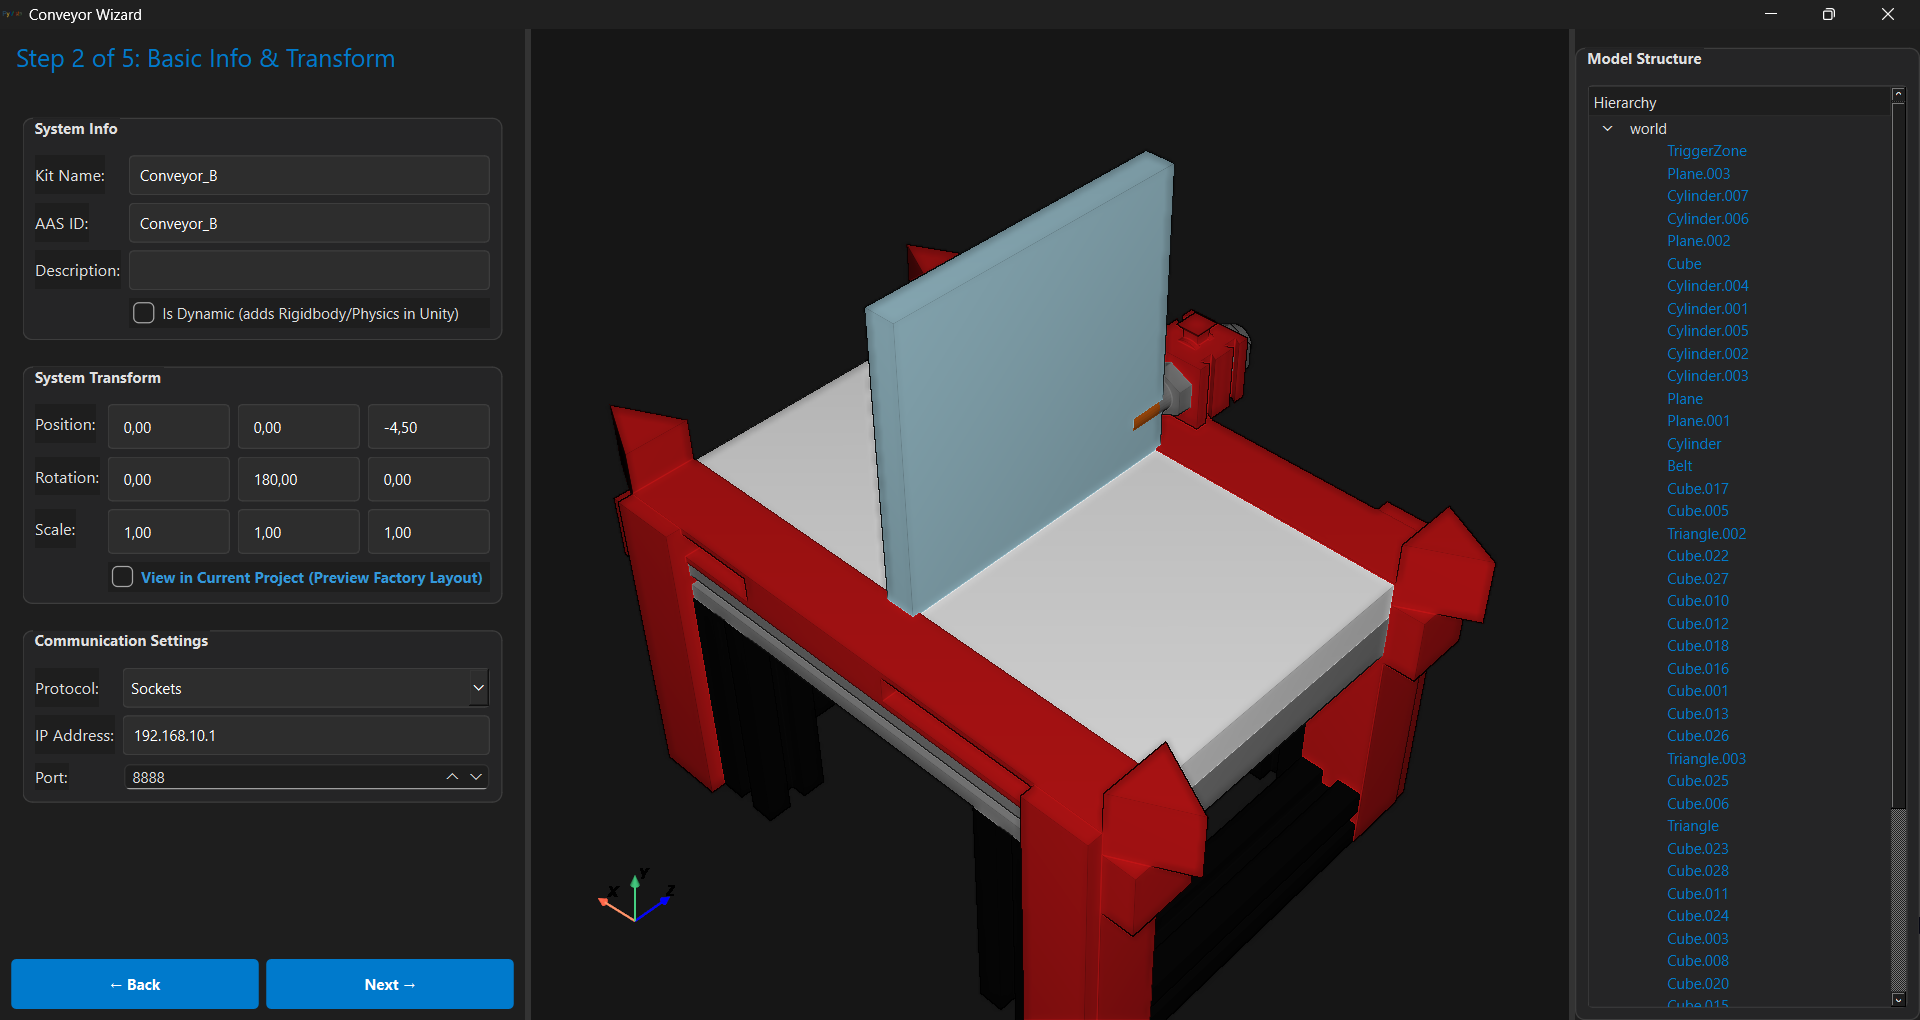
\includegraphics[width=\linewidth,keepaspectratio]{5-Figures/asset_modeling_gui.png}
    \caption{Graphical user interface of the Asset Modeling application showing the interactive 3D viewport, configuration panels, and model structure hierarchy.}
    \label{fig:conveyor_wizard_gui_screenshot}
\end{figure}

As shown in \Cref{fig:conveyor_wizard_gui_screenshot}, the interface is organized into distinct panels designed to guide the user through a structured configuration pipeline:
\begin{itemize}
    \item \textbf{Interactive 3D Viewport (Center):} Displays the imported 3D CAD model with real-time rendering, orbit/pan controls, and visual representation of placed sensor/actuator pins and coordinate frames.
    \item \textbf{Step-by-Step Configuration Wizard (Left Panel):} Guides the engineer through sequential setup tabs to fully populate the submodels:
    \begin{enumerate}
        \item \textit{Model Selection (Step 1):} Selects the asset type and loads the target CAD geometry into the central 3D viewport.
        \item \textit{Basic Info \& Transform (Step 2):} Configures primary metadata (AAS ID, asset name, operational description), 3D spatial transformation (position, orientation and scale), and communication endpoints (IP address and port).
        \item \textit{Configure Sensors (Step 3):} Interactively places virtual sensor pins on the 3D surface using raycasting and defines their operational parameters.
        \item \textit{Configure Actuators (Step 4):} Defines virtual actuator pins, mapping their motion parameters, direction vectors, and actuation modes onto specific mesh nodes.
        \item \textit{Review \& Deploy (Step 5):} Reviews the complete generated submodel hierarchy, previews the structured \gls{JSON} manifest, and deploys the generated .aasx package to the target server or repository.
    \end{enumerate}
    \item \textbf{Model Structure Hierarchy (Right Panel):} Provides a tree view of the asset's internal mesh nodes, allowing engineers to select specific components and inspect geometry hierarchies.
\end{itemize}

\subsection{Interactive Modeling Workflow and Surface Raycasting}
Placing a sensor or actuator pin on the model is done by clicking directly on the 3D mesh surface rather than typing in names or IDs manually. This satisfies requirement \textbf{FR2} (Self-Describing Asset Packages) and eliminates a major source of human error.

When the user clicks on the 3D viewport, an interactive ray is cast from the camera coordinate through the clicked pixel into the scene. The raycasting engine calculates the exact 3D intersection point on the mesh surface, along with the corresponding surface normal vector. The surface normal vector automatically establishes the spatial orientation of the pin, ensuring that sensors placed on inclined or vertical surfaces point in the correct direction.

The complete interactive modeling sequence and workflow between the engineer, the desktop \gls{GUI}, the 3D Viewport, and the \gls{AAS} Data Model are formally depicted in \Cref{fig:wizard_ui}.

\begin{figure}[htbp]
    \centering
    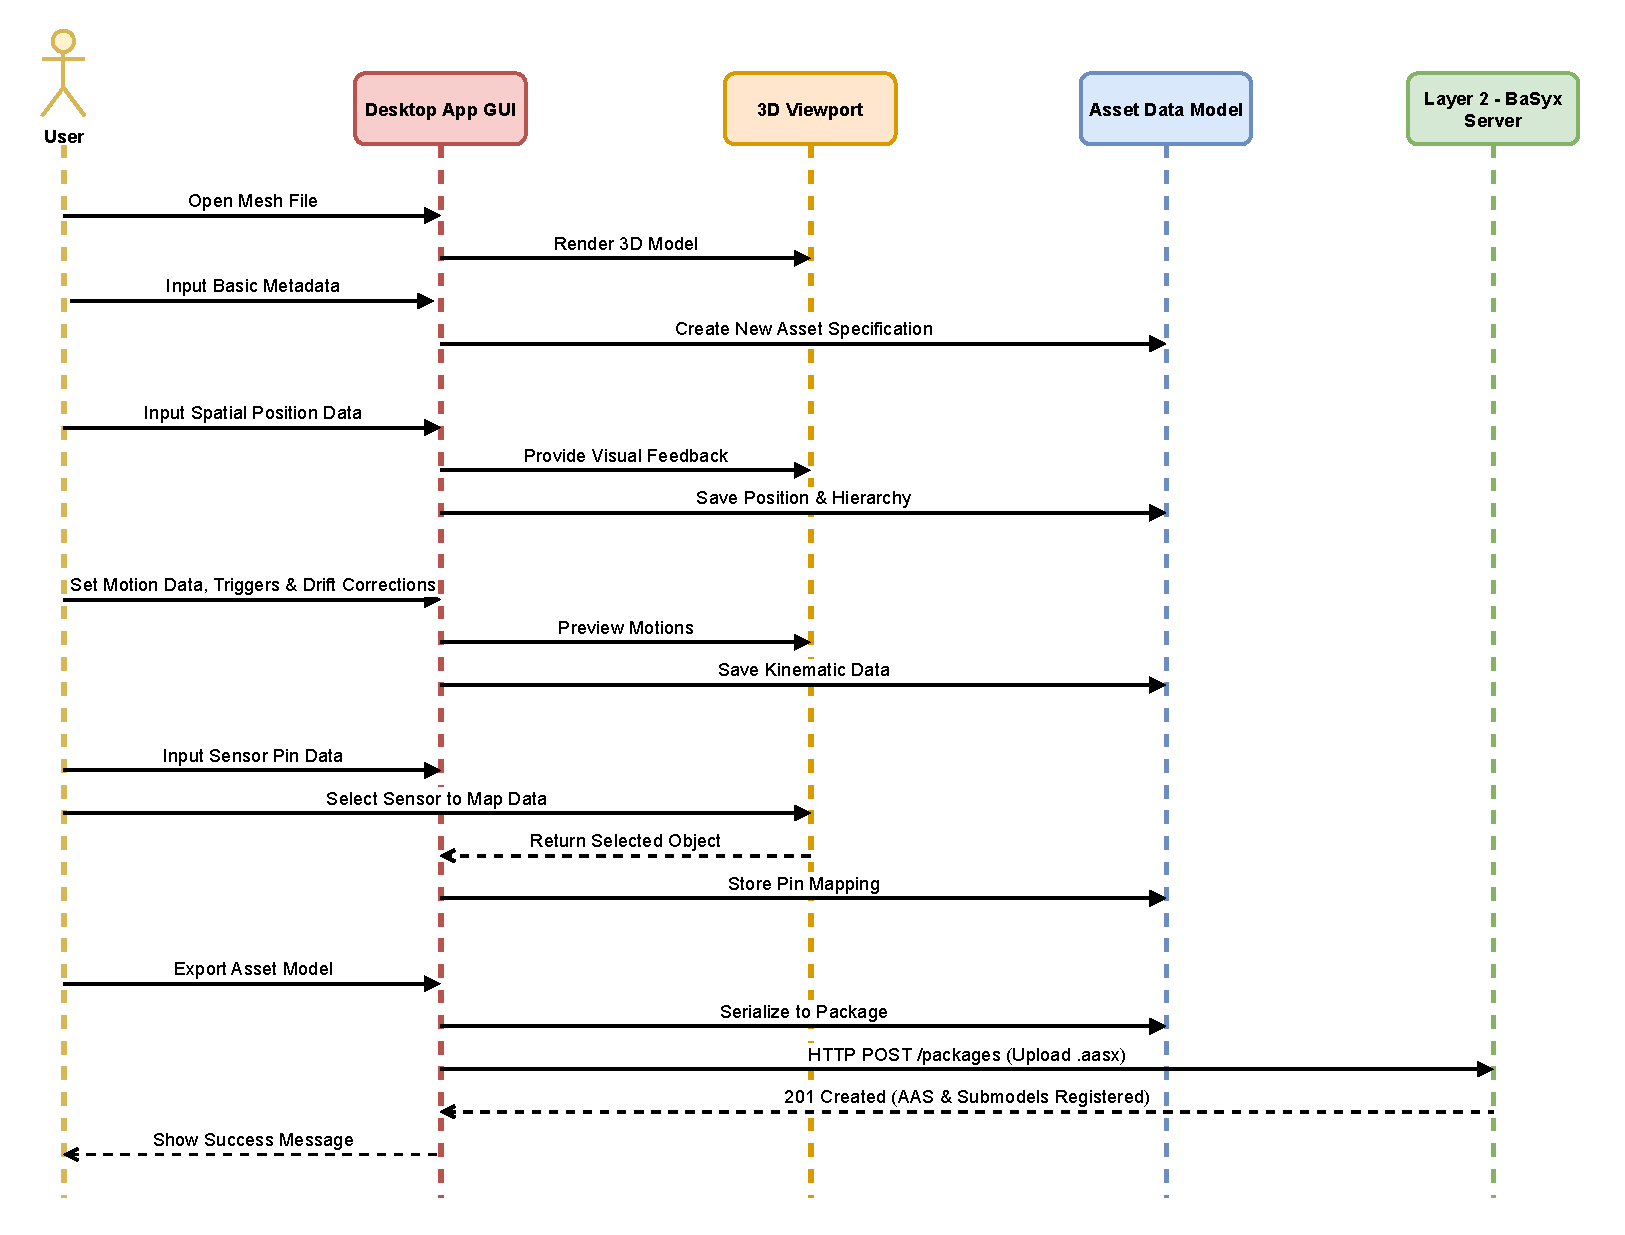
\includegraphics[width=\linewidth,height=0.72\textheight,keepaspectratio]{5-Figures/sequence_layer1.drawio.pdf}
    \caption{\gls{UML} Sequence Diagram depicting the interactive modeling workflow and data model population of Layer 1.}
    \label{fig:wizard_ui}
\end{figure}

\subsection{Integrated Rule Editor for Control Logic}
To enhance physical-digital synchronization and enable closed-loop testing during \gls{VC}, the application includes a dedicated \textit{ControlLogic} rule editor. In line with the non-programmer requirement (\textbf{NFR4}: Configuration Accessibility), the interface provides an intuitive environment that allows domain engineers to program complex interlock sequences without writing code. Engineers define conditional statements evaluating field sensor trigger states and command actuator actions (\Cref{fig:rule_editor_ui}).

\begin{figure}[htbp]
    \centering
    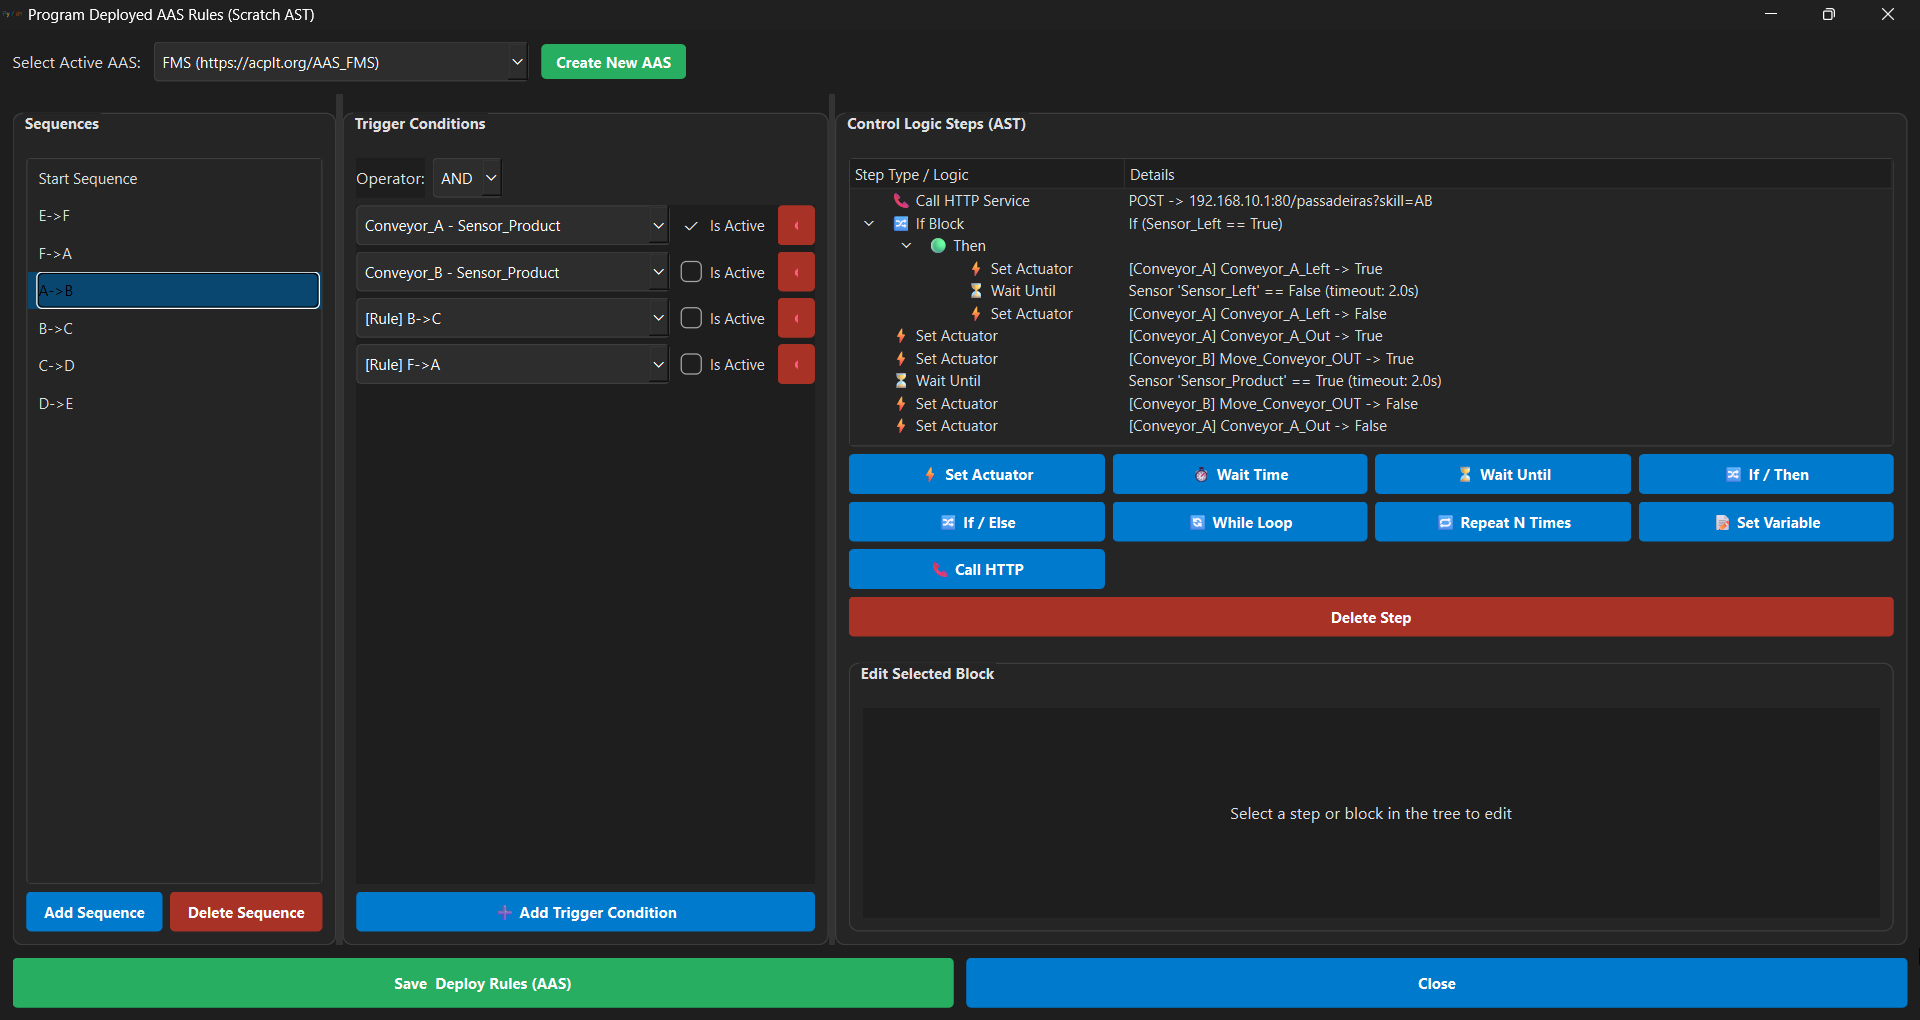
\includegraphics[width=\textwidth,keepaspectratio]{5-Figures/rule_editor_gui.png}
    \caption{User interface of the no-code \textit{ControlLogic} rule editor.}
    \label{fig:rule_editor_ui}
\end{figure}

To construct control sequences visually, the editor provides nine modular block action types that assemble the \gls{AST}:
\begin{itemize}
    \item \textbf{Set Actuator:} Commands a state change on a target actuator pin or relay.
    \item \textbf{Wait Time:} Introduces a fixed time delay (in seconds) before advancing to the next execution step.
    \item \textbf{Wait Until:} Pauses execution until a specific sensor input condition is satisfied or a configurable timeout is reached.
    \item \textbf{If / Then:} Evaluates a boolean sensor condition and executes the nested child steps when true.
    \item \textbf{If / Else:} Provides dual-branch conditional logic, executing the primary sequence if true or an alternative branch if false.
    \item \textbf{While Loop:} Continuously repeats a block of actions as long as the specified sensor condition remains active.
    \item \textbf{Repeat N Times:} Iterates a designated sequence of actions for a fixed integer number of cycles ($N$).
    \item \textbf{Set Variable:} Modifies or initializes an internal runtime state variable used across sequence conditions.
    \item \textbf{Call HTTP:} Dispatches an outbound \gls{HTTP} \gls{REST} request to execute external skills or communicate directly with network controllers.
\end{itemize}

These rules are serialized as structured \glspl{AST} within the \gls{AAS} \textit{ControlLogic} submodel, enabling Unity's local rule engine to validate simulation behavior and maintain tight synchronization with physical shop-floor operations directly from the \gls{AAS} package. \Cref{fig:sequence_rules} illustrates the \gls{UML} sequence diagram of the rule configuration and deployment workflow between the engineer, the Rule Editor \gls{GUI}, the local asset data model, and the Layer~2 BaSyx repository.

\begin{figure}[htbp]
    \centering
    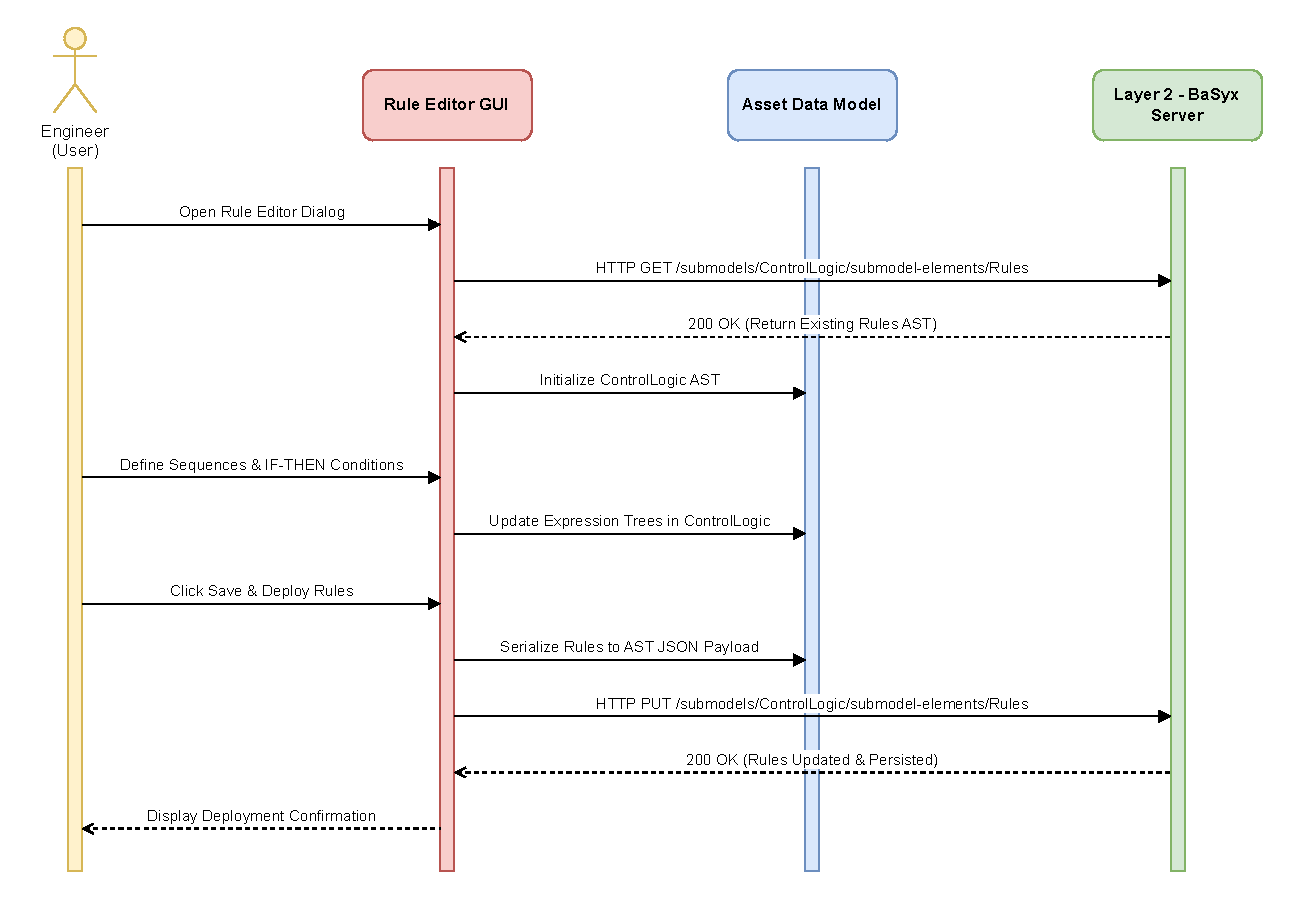
\includegraphics[width=\linewidth,height=0.72\textheight,keepaspectratio]{5-Figures/sequence_rules.drawio.pdf}
    \caption{\gls{UML} Sequence Diagram of the \textit{ControlLogic} rule configuration and deployment workflow.}
    \label{fig:sequence_rules}
\end{figure}

\subsection{AASX Package Generation and Layer 2 Repository Upload}
Once all submodel properties are specified, the application uses the \texttt{basyx-python-sdk} to build the formal AASX package. The 3D GLB geometry is stored as an embedded binary \texttt{Blob}, while the five submodels are serialized into OPC-compliant \gls{JSON} manifests. Finally, the application validates package integrity and publishes the complete AASX bundle to the Layer~2 BaSyx repository via \gls{REST} endpoints.

\section{Layer 2: Storage and Registry (Eclipse BaSyx v2)}
\label{sec:impl_basyx}

Layer~2 runs on Eclipse BaSyx~v2, deployed as a set of Docker Compose containers inside an isolated network. Docker was chosen because it makes the entire containerized server stack reproducible: a single \texttt{docker compose up} command starts all services in the correct order with no manual configuration. This setup allows new asset submodels and associated services to be instantiated upon startup, fulfilling requirement \textbf{FR1} (Plug-and-Play Asset Onboarding).

\Cref{fig:component_layer2} shows the component structure and service interfaces of Layer~2, which centers on five core components. The \gls{AAS} Environment Repository stores uploaded AASX packages, handling package ingestion, web inspection, and model retrieval for Unity simulation clients. The \gls{AAS} Registry and Submodel Registry manage registered shells and submodel URLs, respectively, exposing endpoints for registration, discovery, and lookup. Internal persistence across all registries and repositories is backed by a shared MongoDB database. Finally, operators can inspect and browse all live machines through the BaSyx Web \gls{GUI} using the catalog and submodel browsing endpoints.

\begin{figure}[htbp]
    \centering
    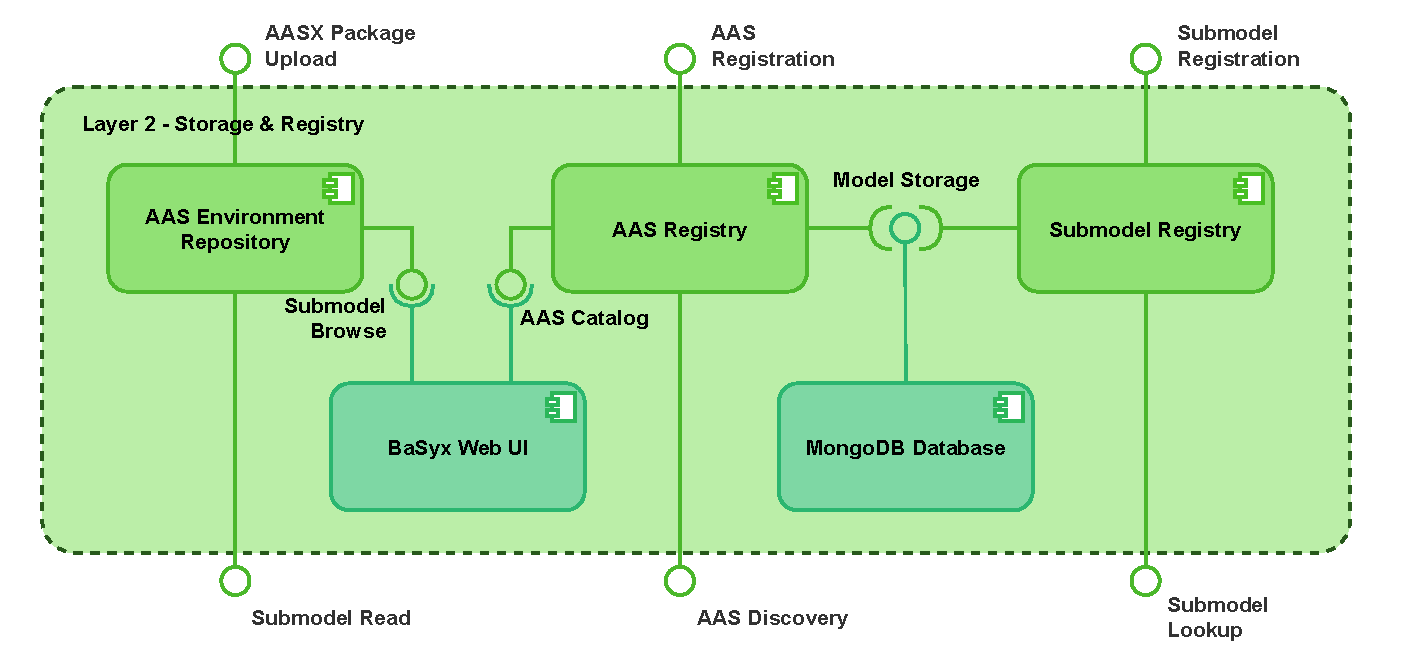
\includegraphics[width=\linewidth,height=0.72\textheight,keepaspectratio]{5-Figures/Layer 2 - Storage & Registry.pdf}
    \caption{Component architecture and interface boundaries of Layer 2 (Storage and Registry).}
    \label{fig:component_layer2}
\end{figure}

The container networking and service topology is illustrated in \Cref{fig:basyx_docker_topology}.

\begin{figure}[htbp]
    \centering
    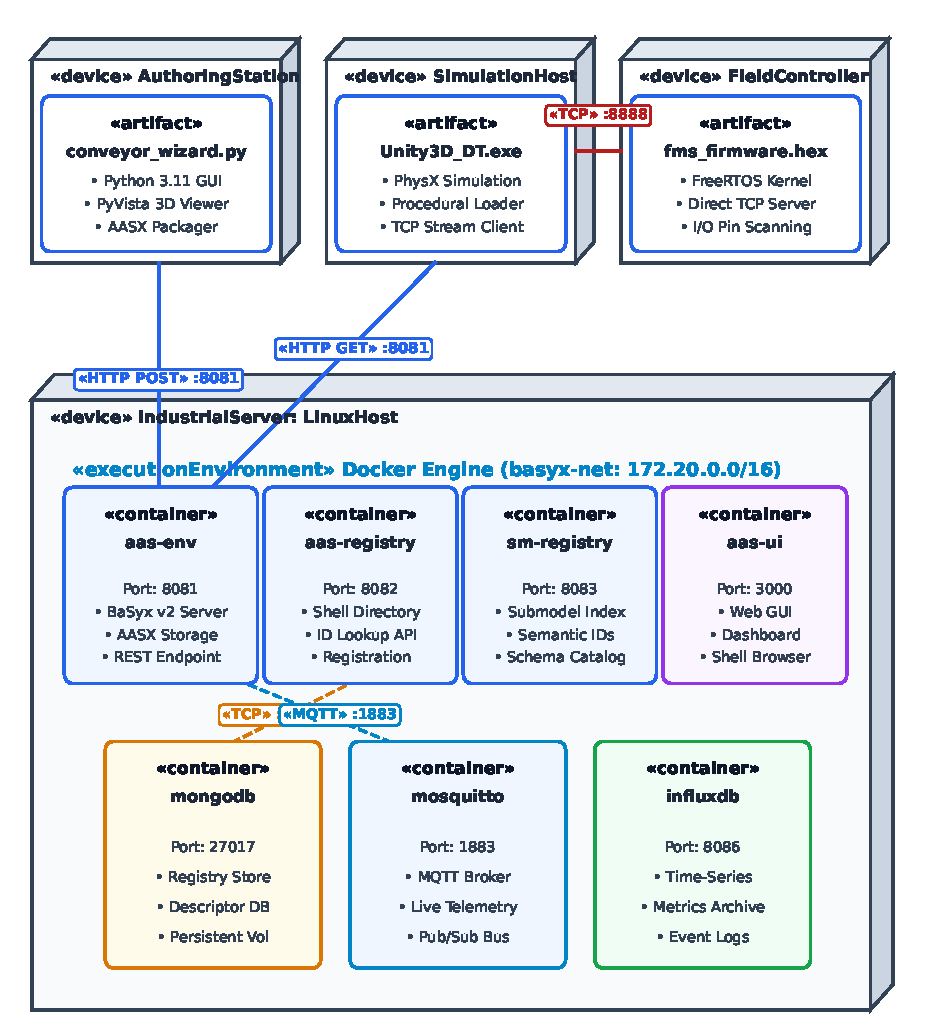
\includegraphics[width=0.8\textwidth]{5-Figures/basyx_docker_topology.pdf}
    \caption{Container networking and service topology of the Eclipse BaSyx v2 Docker deployment.}
    \label{fig:basyx_docker_topology}
\end{figure}

\subsection{Microservice Architecture and Port Allocation}
The containerized services provide the repository and registry functions defined in \Cref{fig:activity_layer2}. The \gls{AAS} Environment Repository (port 8081) exposes standard \gls{REST} endpoints to store and serve \gls{AAS} packages, submodels, and 3D mesh files. The \gls{AAS} Registry (port 8082) and Submodel Registry (port 8083) maintain directory indices of active assets, resolving unique asset identifiers to live \gls{HTTP} network endpoints. Persistent storage for shell metadata, submodels, and descriptors is maintained by a shared MongoDB instance (port 27017). By decoupling storage across microservices, Layer~2 scales as additional machines and simulation clients are added to the network, satisfying requirement \textbf{NFR2} (Scalability). Although the standard BaSyx~v2 deployment stack includes an Eclipse Mosquitto \gls{MQTT} Broker (port 1883) and an InfluxDB time-series database (port 8086), real-time synchronization in this work bypasses \gls{MQTT} event streaming in favor of direct low-latency \gls{TCP} socket communication with the field \gls{PLC}, minimizing end-to-end telemetry delay. Operators can interact with and inspect the entire live deployment through the BaSyx Web \gls{GUI} dashboard (port 3000).

\subsection{Package Ingestion and Registry Resolution}
When an AASX package is uploaded via \gls{HTTP} POST to port 8081 at the upload endpoint, the repository extracts its contents. 3D meshes (GLB) are placed in the static web server directory, accessible via standard URLs, while shell metadata and submodels are stored in MongoDB.

Next, registration calls are sent to both the \gls{AAS} Registry (shell descriptors on port 8082) and the Submodel Registry (submodel descriptors on port 8083). These records publish the asset ID, short name, and \gls{REST} endpoint URLs. Simulation clients can then discover available machines and their submodels with a single query.

\section{Layer 3: Runtime Execution and Physical Synchronization}
\label{sec:impl_unity}

The Runtime Execution and Physical Synchronization layer (\Cref{sec:layer3_conceptual}) connects Unity 3D with the physical testbed through collaborating components shown in \Cref{fig:component_layer3}. At the simulation core, the main orchestrator downloads model packages from Layer~2 and instantiates virtual equipment into the scene. The asset importer inspects model descriptors and binds runtime scripts to corresponding scene nodes. Virtual sensor signals and kinematic motor commands are processed by the sensor and actuator controllers, while the rule engine evaluates local conditional logic during virtual testing without requiring physical controllers. Workpiece dynamics are managed by the dynamic product controller, which applies position corrections to eliminate physical drift. Runtime execution modes are coordinated by the operation mode manager alongside the hardware telemetry link, which ingests raw telemetry over \gls{TCP} and triggers motor routines via \gls{HTTP}. Finally, on the shop floor, the Industrial Shields M-DUINO \gls{PLC} reads 24\,V sensor inputs through optocouplers and triggers relay outputs to operate the conveyor motors. This complete architectural separation ensures that updates or failures in individual layers do not propagate, enforcing requirement \textbf{NFR3} (Layer Independence).

\begin{figure}[htbp]
    \centering
    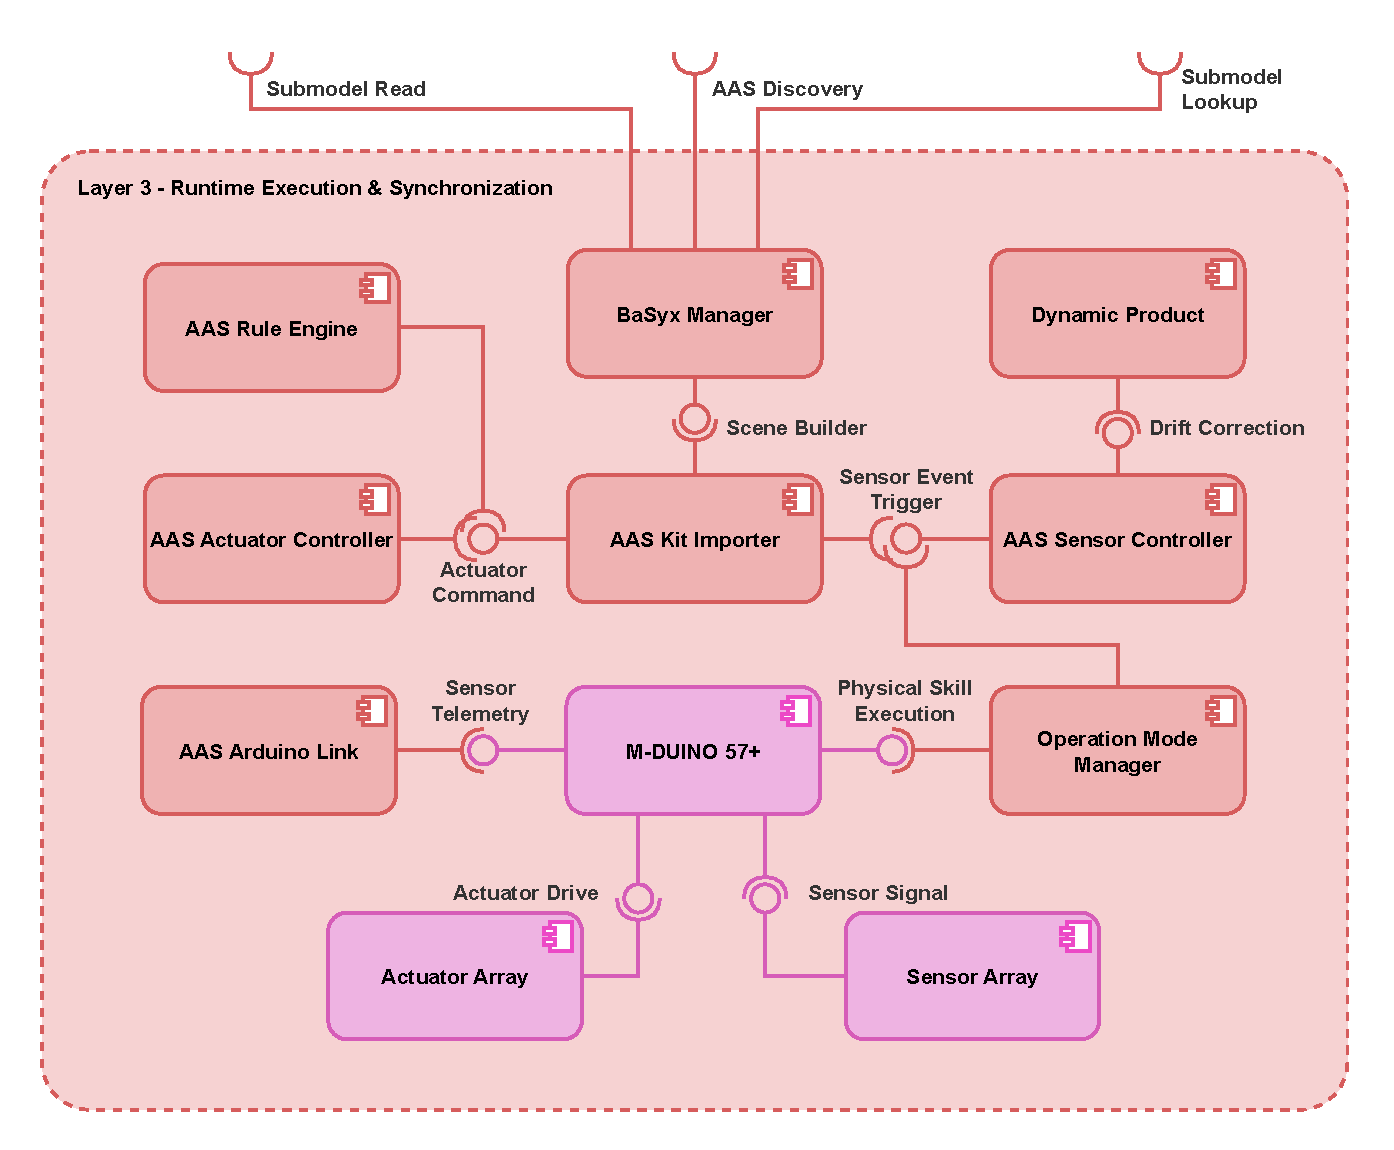
\includegraphics[width=\linewidth,height=0.72\textheight,keepaspectratio]{5-Figures/Layer 3 - Runtime Execution & Synchronization.pdf}
    \caption{Component architecture and interface boundaries of Layer 3 (Runtime Execution and Physical Synchronization).}
    \label{fig:component_layer3}
\end{figure}

\subsection{Dynamic Ingestion Flow and Procedural Scene Construction}
To satisfy requirement \textbf{FR3} (Dynamic Scene Assembly) and support automated onboarding (\textbf{FR1}: Plug-and-Play Asset Onboarding), the Unity virtual environment operates as a standalone executable that constructs the scene procedurally upon launch without needing pre-saved scene files. The execution flow follows the \gls{UML} sequence diagram presented later in \Cref{fig:unity_runtime_sequence}, which structures the runtime lifecycle across three main phases:

\begin{enumerate}
    \item \textbf{Phase 1: Registry Discovery and Cache Clearing.} At startup, the singleton orchestrator purges stale local mesh files from the disk cache. It then sends an \gls{HTTP} GET request to the BaSyx \gls{AAS} Registry on port 8082. Upon receiving the array of active shell descriptors, it deserializes the \gls{JSON} payload and launches an asynchronous ingestion worker for each discovered machine asset.
    \item \textbf{Phase 2: Procedural Import, Mesh Normalization, and Physics Setup.} For each asset, the importer queries the repository on port 8081 to retrieve the visual structure, virtual pins, behavior mapping, and control logic submodels, alongside streaming the 3D mesh GLB file. Using glTFast, Unity procedurally instantiates the 3D scene hierarchy. To reconcile Blender's right-handed coordinate system with Unity's left-handed space, a $180^\circ$ Y-axis rotation is applied. Finally, hierarchy normalization bakes non-uniform scales directly into the mesh vertices to prevent rotational shearing, and binds sensor and actuator controllers to map virtual input and output terminals.
    \item \textbf{Phase 3: Dual-Mode Execution and Telemetry Loop.} After a stabilization delay for PhysX dynamics and output registers to settle, the runtime enters active execution in one of two modes:
    \begin{itemize}
        \item \textbf{Mode A (\gls{VC}):} The orchestrator initializes all queued rule engines, parsing the IF-THEN rules from the control logic submodels. When a virtual product triggers a sensor collider, the sensor controller emits a state change notification. The rule engine evaluates the logic tree and commands the actuator controller to set target motor speeds or actuate pneumatic stoppers in a closed software loop.
        \item \textbf{Mode B (Live \gls{DT} Synchronization):} Local rule evaluation is disabled, and the communication link initiates a multi-threaded \gls{TCP} client connecting to the physical \gls{PLC} on port 8888. A background thread continuously ingests compact telemetry packets, pushing events to a thread-safe queue. When dequeued on the main thread, port callbacks update virtual sensor \gls{UI} highlights and prompt kinematic position snapping in the dynamic product controller, while asynchronous \gls{HTTP} PUT calls update live property values in the BaSyx repository.
    \end{itemize}
\end{enumerate}

\subsection{Conveyor Physics Simulation}
To ensure physical realism, conveyor belts are simulated using PhysX friction and surface velocity vectors rather than simple translation scripts. By setting a tangential surface velocity on conveyor colliders, products experience realistic friction, inertia, acceleration, and contact forces. The implementation relies on two cooperating components: the surface script attached to the conveyor collider to assign friction parameters and linear velocity along the belt axis, and the contact tracker component attached dynamically to products marked with the dynamic product tag to track active contact points and impart drive forces.

\subsection{Dual-Mode Execution Framework}
\label{sec:impl_dual_mode}

To support different stages of engineering, the runtime provides two operating modes, as shown in \Cref{fig:unity_runtime_sequence}. Mode~A (\gls{VC}) (when DIGITAL TWIN = FALSE) validates system behavior before physical hardware is connected. When a simulated product triggers a virtual sensor, the physics proxy updates the local sensor state and alerts the sensor controller. The rule engine then evaluates the IF-THEN rules from the control logic submodel, driving virtual actuators in a closed loop entirely within the simulation engine. Conversely, Mode~B (Live \gls{DT} Synchronization) (when DIGITAL TWIN = TRUE) operates during live plant execution. In this mode, rule evaluation is disabled, and the hardware telemetry link connects directly to the physical \gls{PLC} over a low-latency \gls{TCP} socket on port 8888. Incoming sensor telemetry immediately updates virtual sensor states and prompts kinematic snapping in the dynamic product controller, while asynchronous \gls{HTTP} calls keep the BaSyx repository synchronized with physical shop-floor events.

\begin{figure}[htbp]
    \centering
    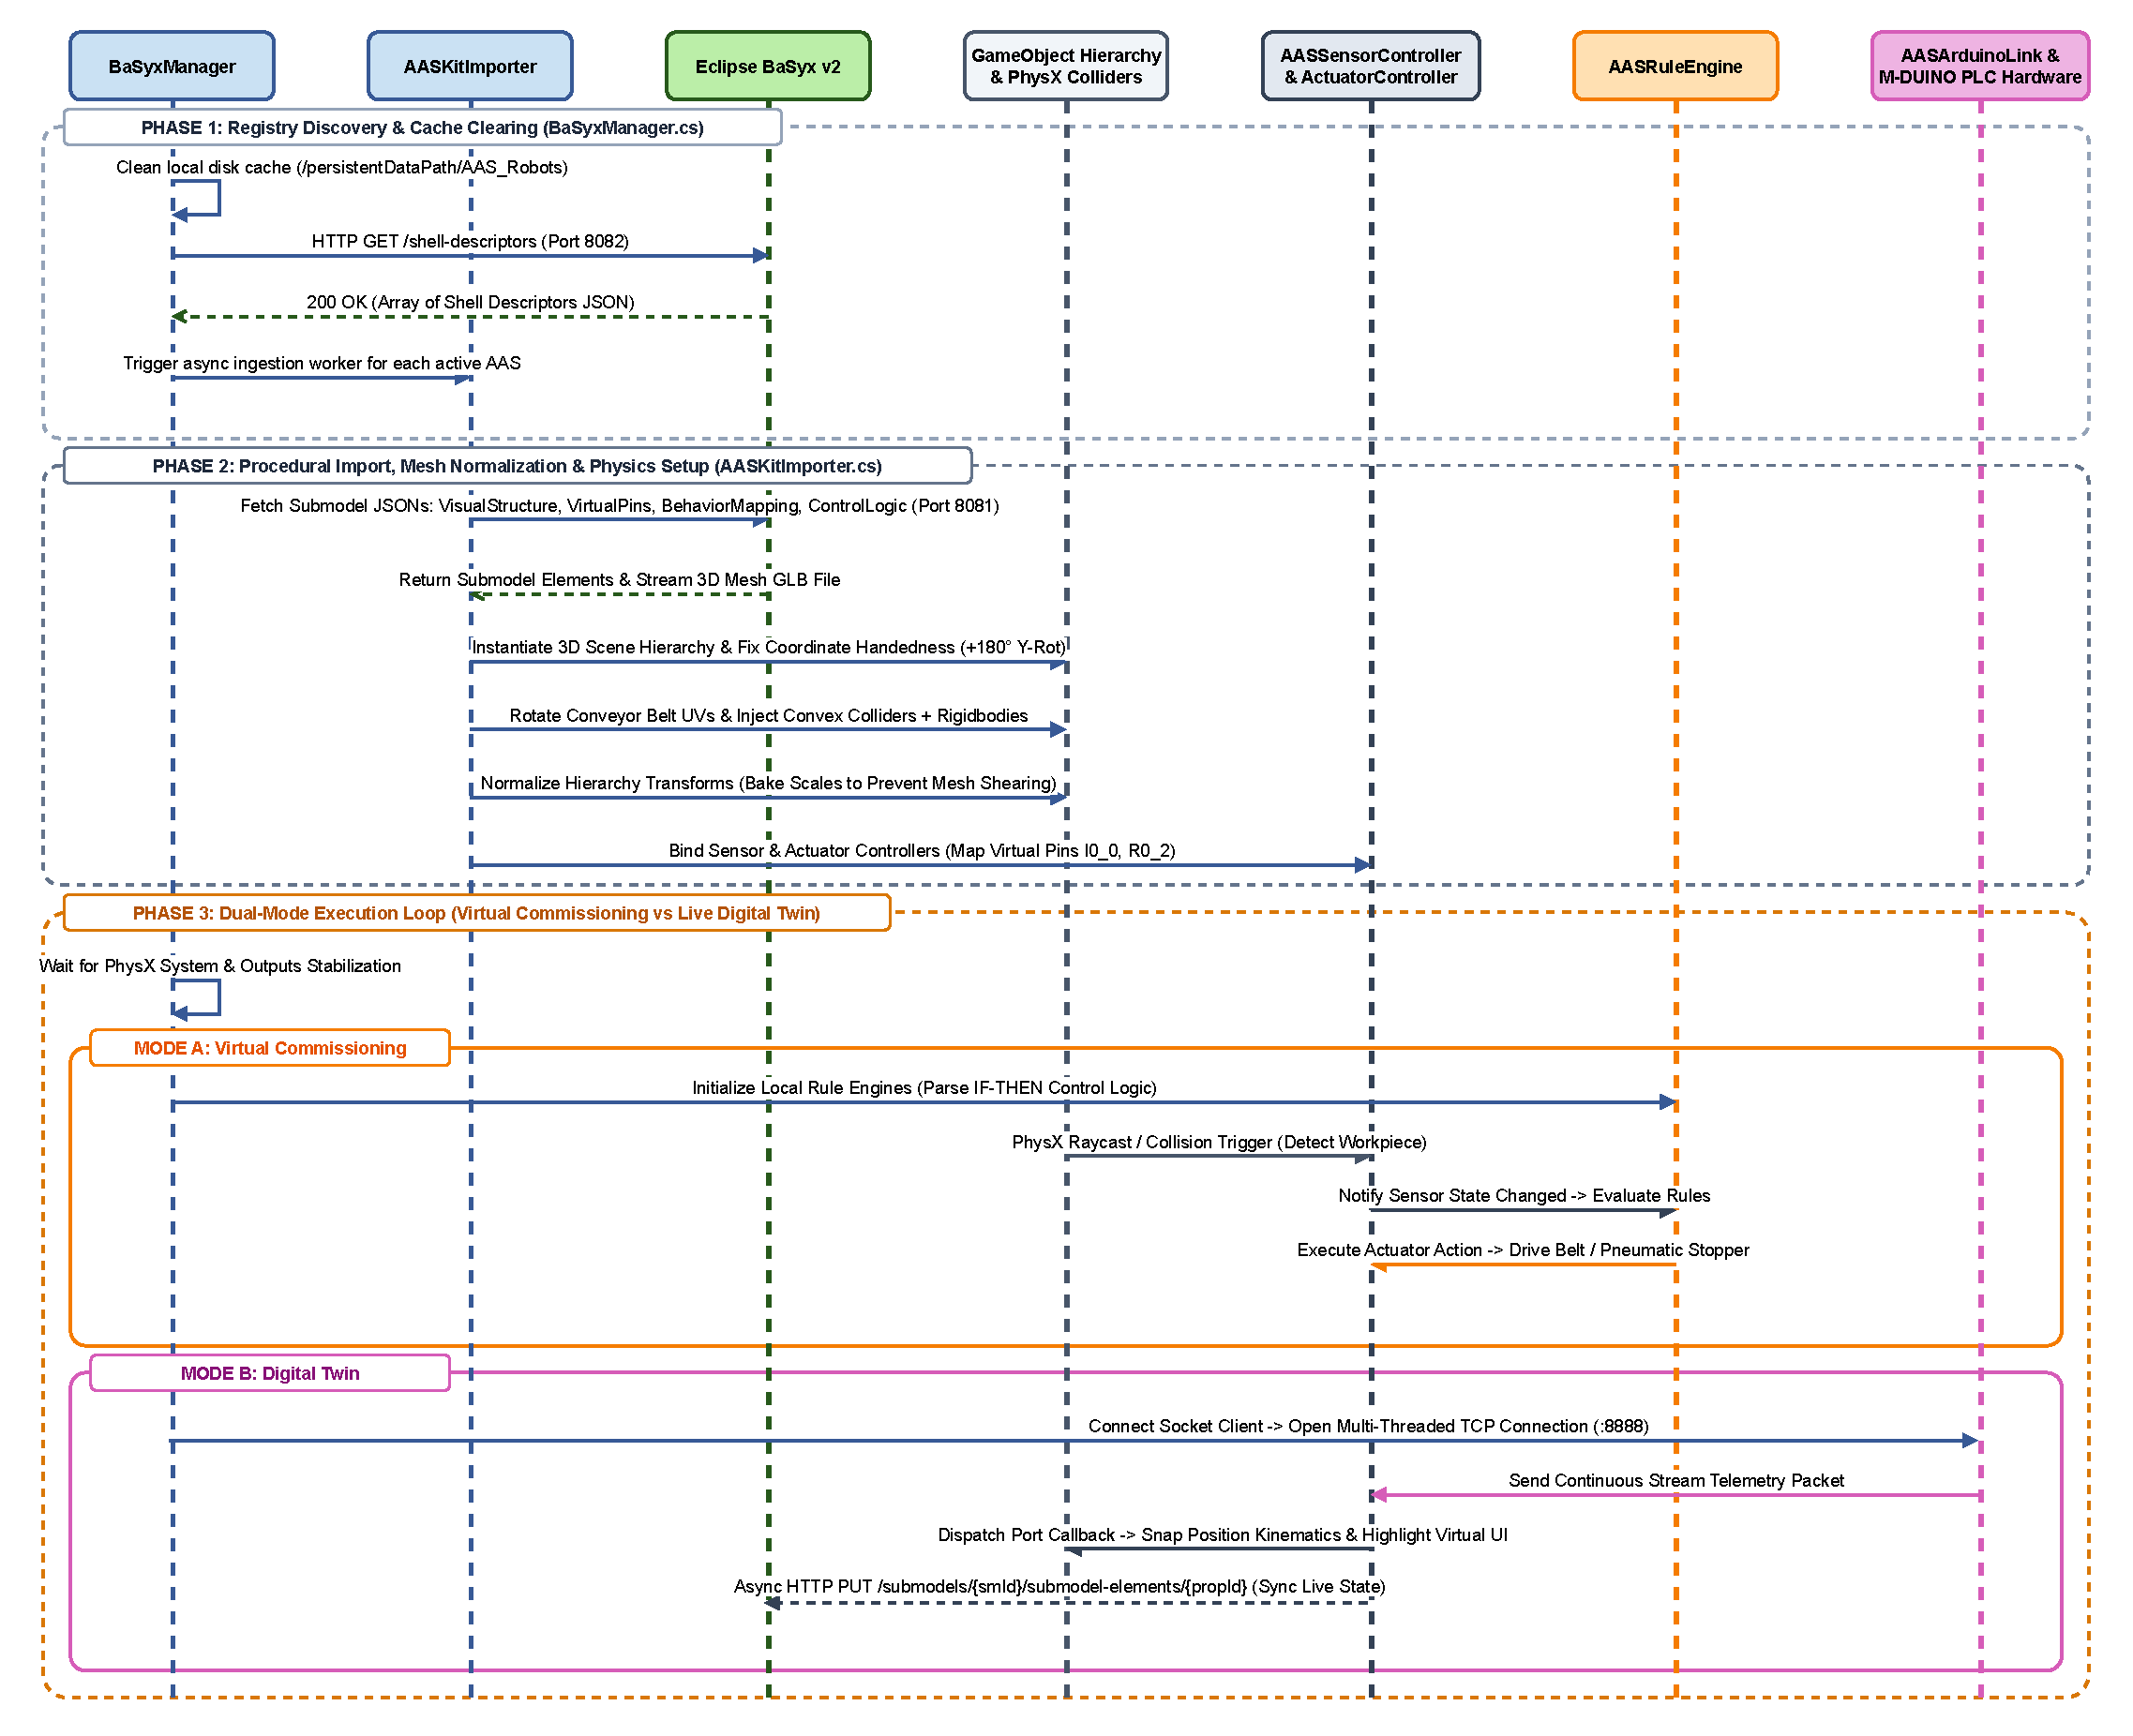
\includegraphics[width=\linewidth,height=0.75\textheight,keepaspectratio]{5-Figures/unity_runtime_sequence.pdf}
    \caption{\gls{UML} Sequence Diagram of the Unity 3D runtime execution environment.}
    \label{fig:unity_runtime_sequence}
\end{figure}

\subsection{Kinematic Drift Correction (Snapping)}
\label{sec:impl_snapping}
Due to continuous numerical physics calculations and small network delays, the simulated product position can slowly drift away from the physical product over time. To preserve synchronization (\textbf{FR4}: Physical-Virtual Synchronization), the dynamic product controller uses a position snapping algorithm. Whenever a physical optical sensor detects a product, the simulation identifies the matching virtual product and moves it to the known 3D position of that physical sensor, removing accumulated drift.

\begin{figure}[htbp]
    \centering
    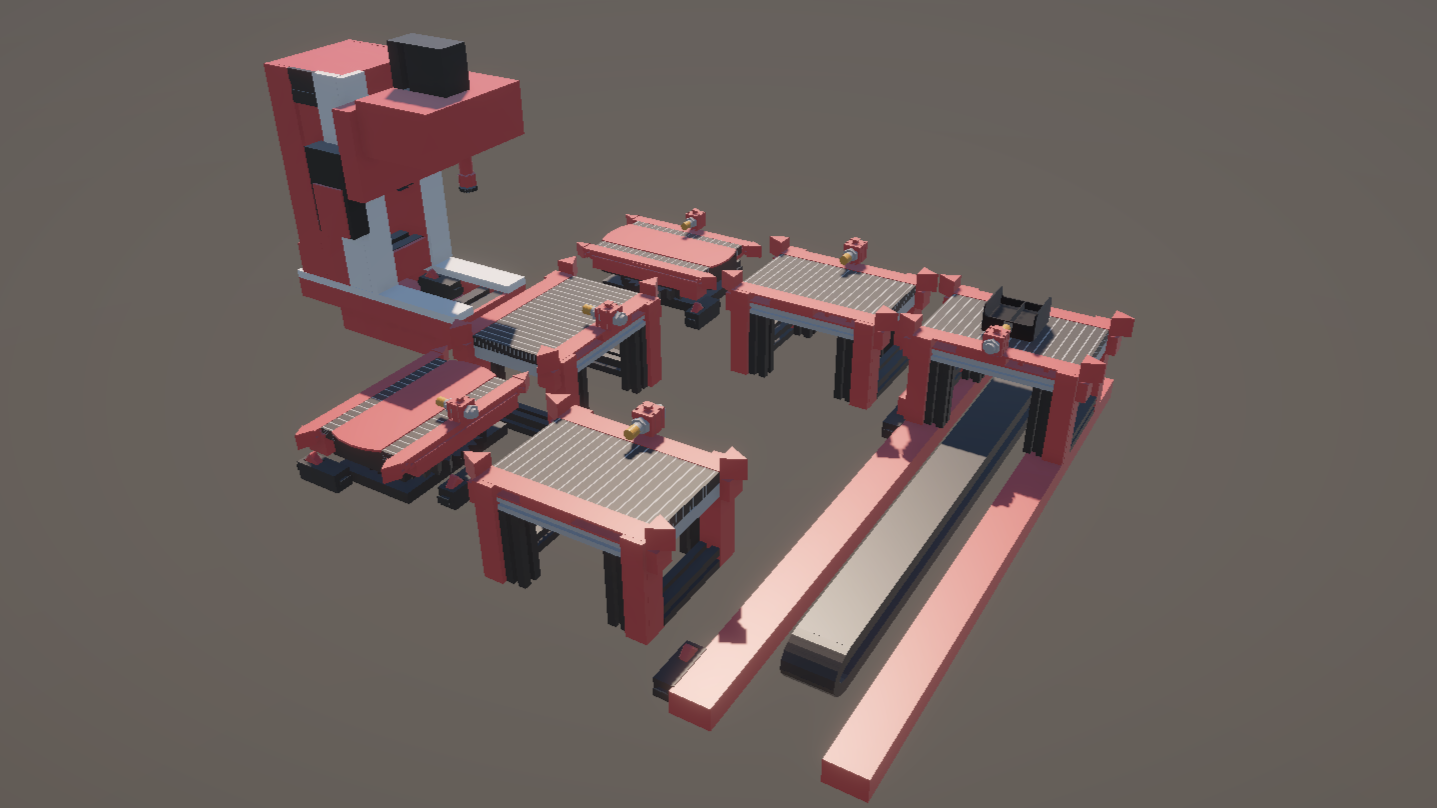
\includegraphics[width=\linewidth,keepaspectratio]{5-Figures/unity_runtime_screenshot.png}
    \caption{3D visualization and \gls{DT} runtime running in Unity 3D.}
    \label{fig:unity_runtime_screenshot}
\end{figure}

\section{Physical Automation Setup and Embedded Firmware}
\label{sec:impl_firmware}

The physical testbed is a modular closed-loop conveyor system. Field control and telemetry dispatching run on an Industrial Shields M-DUINO 57R+ \gls{PLC} (\Cref{fig:physical_hardware_photo}), built around an Arduino Mega 2560 microcontroller equipped with an integrated W5500 Ethernet controller. \Cref{fig:arduino_freertos_schema} illustrates the \gls{UML} sequence diagram of the embedded FreeRTOS firmware execution across hardware initialization, real-time sensor scanning, \gls{IPC} event queuing, \gls{TCP} telemetry streaming, and \gls{HTTP} \gls{REST} actuation channels.

\begin{figure}[htbp]
    \centering
    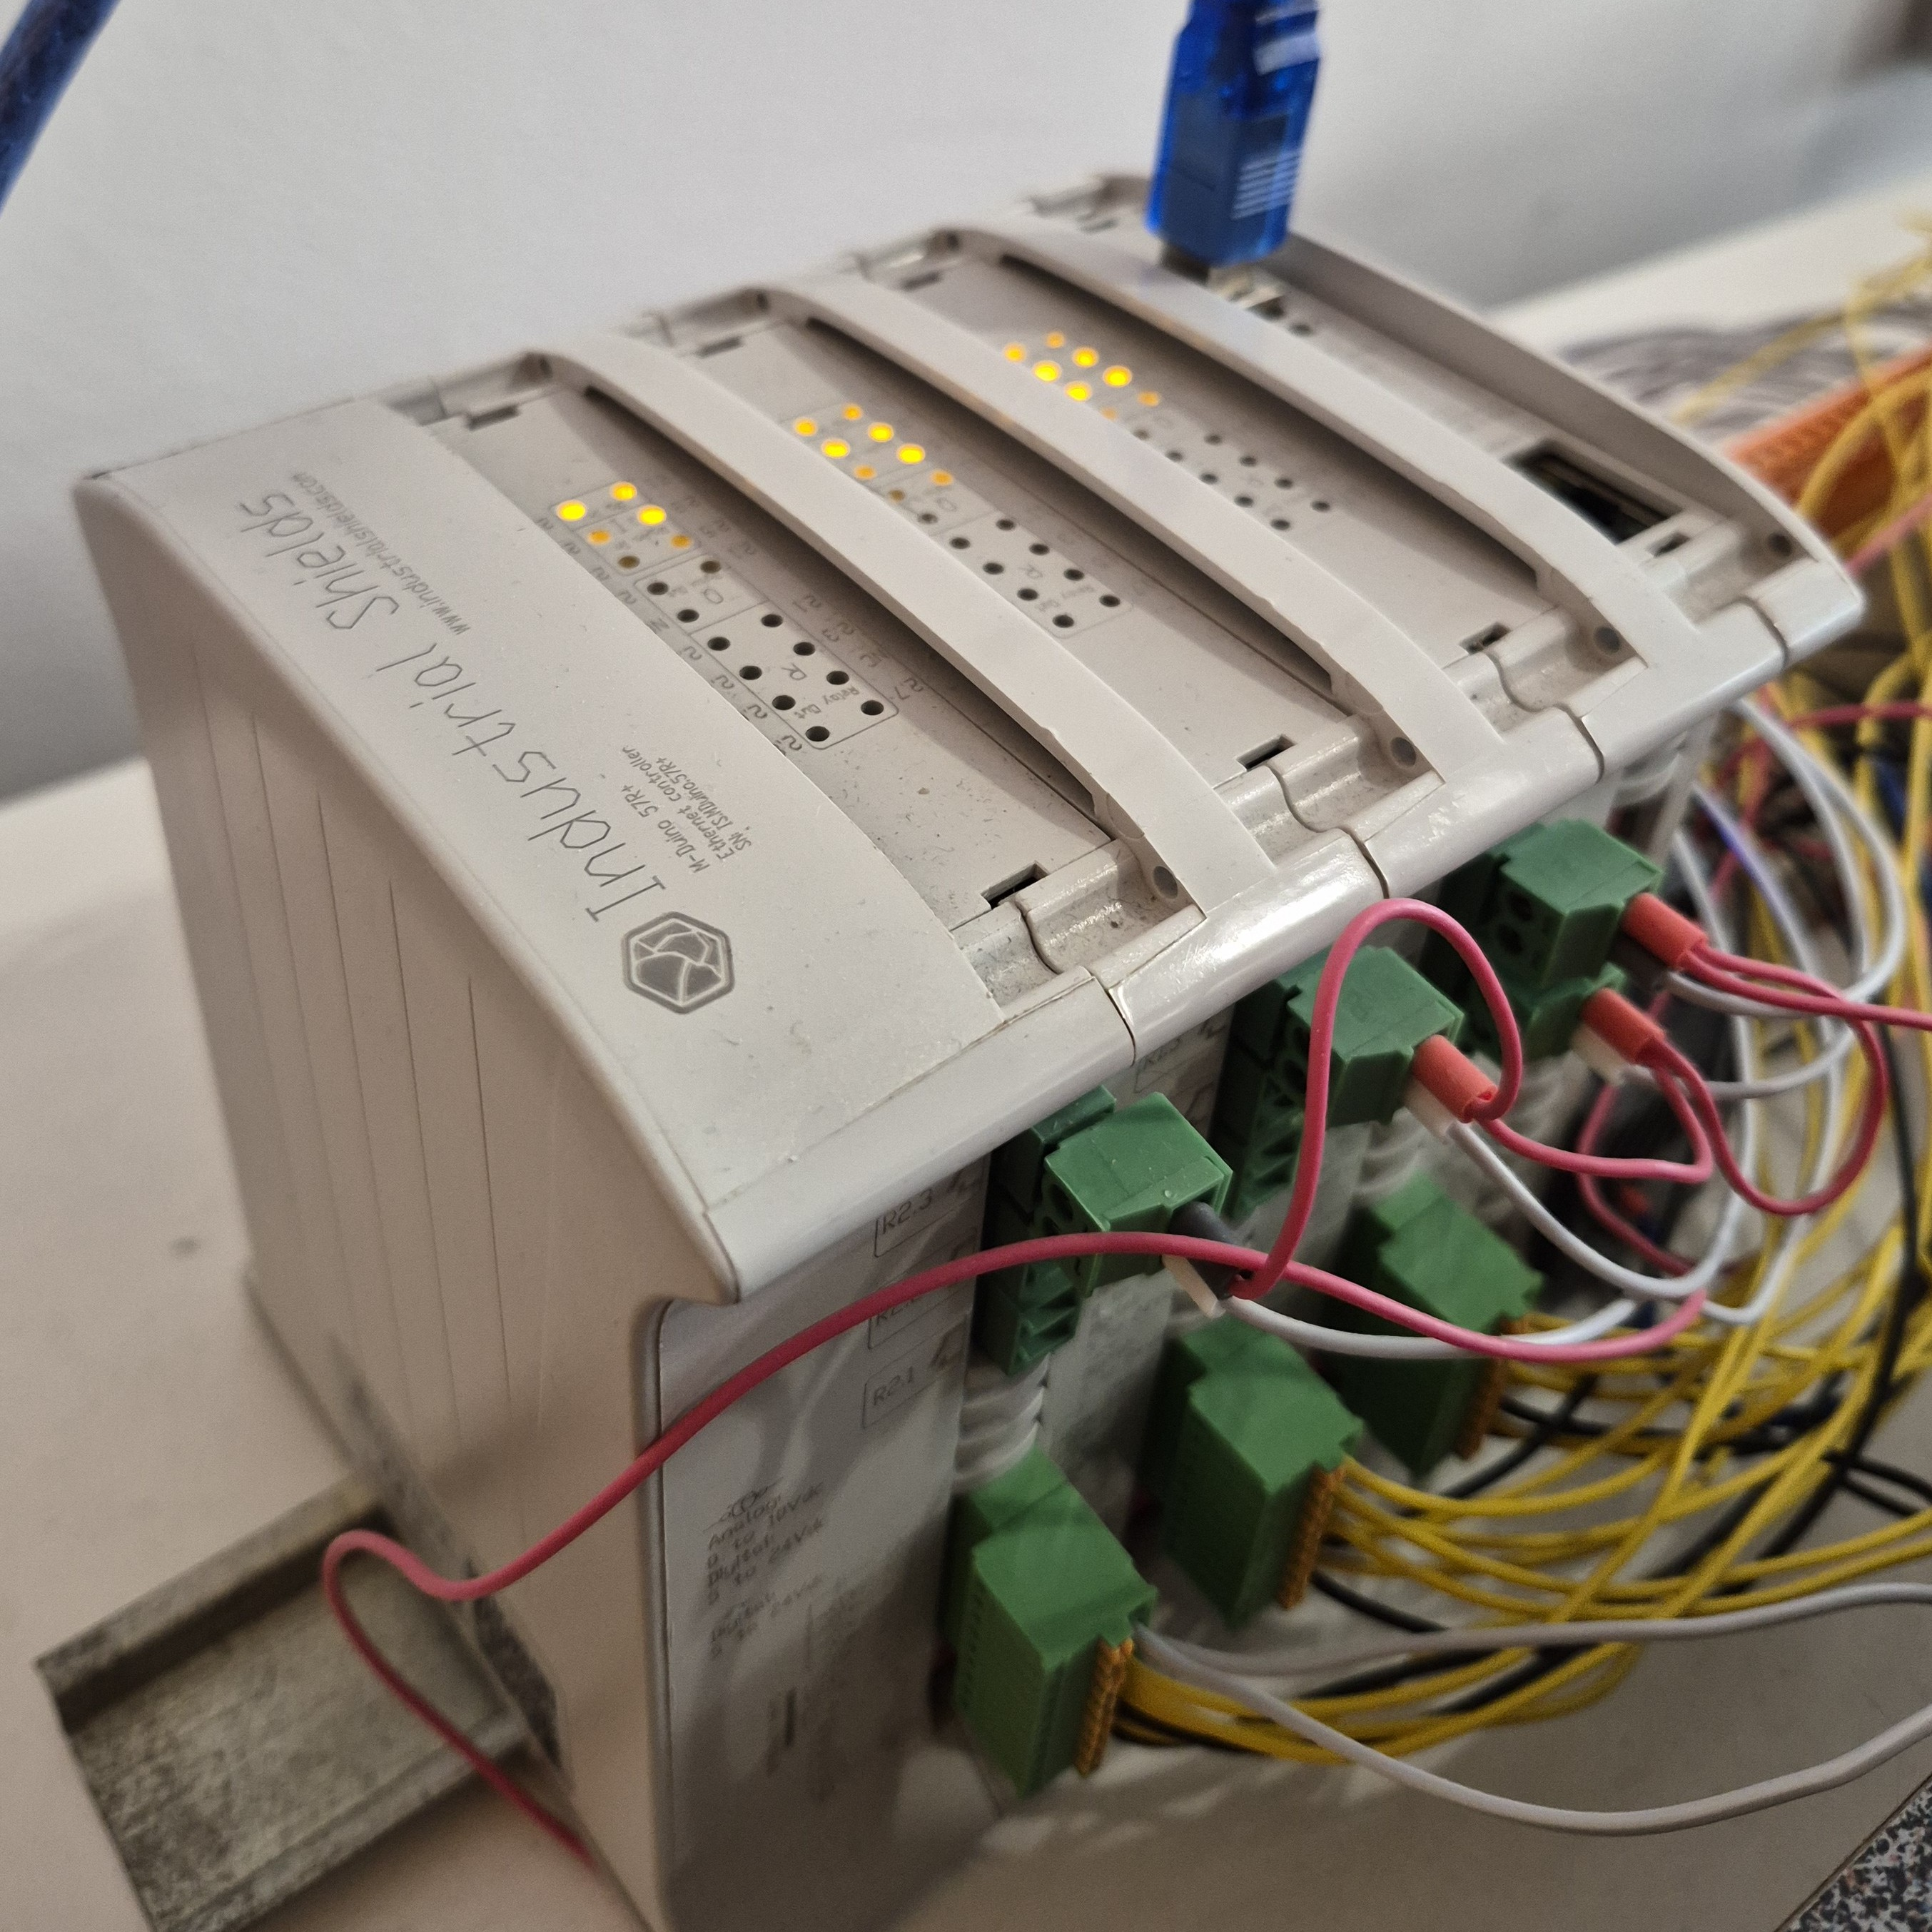
\includegraphics[width=0.65\linewidth,height=0.45\textheight,keepaspectratio]{5-Figures/fms_mduino_plc.jpg}
    \caption{Industrial Shields M-Duino 57R+ \gls{PLC} with DIN-rail mount, field \gls{IO} terminal blocks, and Ethernet and USB interfaces.}
    \label{fig:physical_hardware_photo}
\end{figure}

\begin{figure}[htbp]
    \centering
    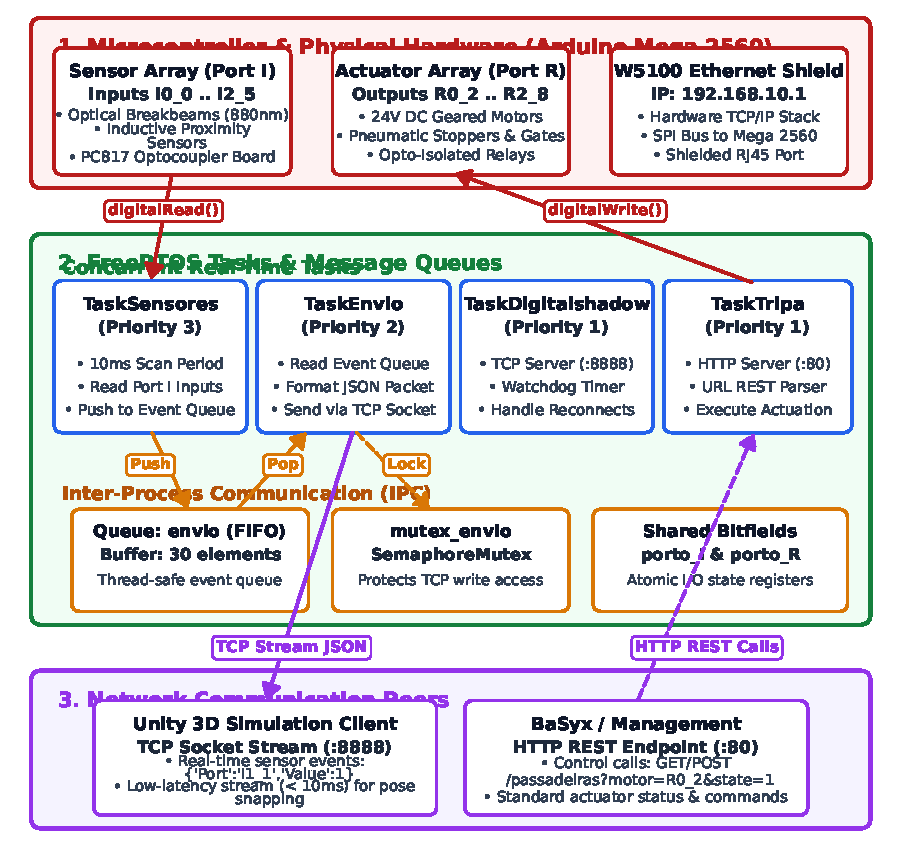
\includegraphics[width=\linewidth,height=0.72\textheight,keepaspectratio]{5-Figures/arduino_freertos_schema.pdf}
    \caption{\gls{UML} Sequence Diagram of the embedded FreeRTOS firmware execution.}
    \label{fig:arduino_freertos_schema}
\end{figure}

\subsection{Sensor Interfacing and Electrical Isolation}
The testbed uses 24\,V~DC optical sensors and inductive proximity detectors. To protect the 5\,V microcontroller logic from voltage spikes and motor electrical noise, all digital inputs pass through optocoupled isolation circuits before reaching the controller \gls{GPIO} pins.

\subsection{FreeRTOS Multi-Tasking Architecture and Procedural Lifecycle}
The firmware runs on the FreeRTOS real-time operating system to guarantee deterministic execution timing and non-blocking network communication across four concurrent tasks. As illustrated in the sequence diagram (\Cref{fig:arduino_freertos_schema}), the operational lifecycle progresses through three distinct functional phases:

\begin{enumerate}
    \item \textbf{Phase 1: Hardware Setup and Dual-Server Initialization.} Upon power-on, the microcontroller executes initial pin configurations, setting input modes for optical sensors and output modes for motor drive relays. It then instantiates the core \gls{IPC} primitives: a 30-element \gls{FIFO} message queue for sensor events and a binary semaphore mutex to prevent race conditions during network socket writes. Finally, the firmware launches two distinct network servers, an \gls{HTTP} server on port 80 and a raw \gls{TCP} socket server on port 8888, before handing control to the FreeRTOS preemptive scheduler to spawn the four real-time tasks.
    \item \textbf{Phase 2: Real-Time Sensor Scanning and Telemetry Dispatching.} The sensor scanner task operates as the highest-priority routine (Priority 3), executing a periodic 5\,ms scan loop across all digital input pins. When an optocoupler signal changes state, the routine applies software debounce filtering. Upon detecting a valid edge transition, it constructs a sensor event token and pushes it onto the thread-safe message queue. This queue insertion unblocks the telemetry stream task (Priority 2), which pops the event token, acquires the network mutex, formats a compact \gls{JSON} telemetry packet, and streams it immediately across the open \gls{TCP} socket (port 8888) to the Unity simulation client.
    \item \textbf{Phase 3: Dual-Channel Actuation Loop and Session Management.} Actuation and management commands follow two dedicated communication pathways. For external control calls (such as skill execution requests from BaSyx or manual operator commands), the \gls{HTTP} server task (Priority 1) receives \gls{REST} requests on port 80, parses target parameters, updates shared output bitfield registers, and triggers the physical opto-isolated relays to drive conveyor motors or pneumatic stoppers. Simultaneously, the session monitor task (Priority 1) maintains \gls{TCP} connection health, executing watchdog checks to recover gracefully from network drops without stalling field control loops.
\end{enumerate}

\subsection{Dual-Channel Communication Strategy}
To support both configuration and real-time synchronization, the firmware implements the dual-channel approach from \Cref{sec:architecture_conceptual}. The administrative and \gls{REST} channel operates on Port~80 via an embedded \gls{HTTP} server, serving on-demand status requests and parameter adjustments. In contrast, the low-latency telemetry channel maintains a dedicated \gls{TCP} socket on Port~8888 implementing the Low-Latency Telemetry Flow (\Cref{sec:architecture_flows}), bypassing \gls{HTTP} parsing overhead to deliver input change events to Unity with minimal latency, satisfying requirement \textbf{NFR1} (Low-Latency Telemetry).

\section{Chapter Summary}
\label{sec:impl_summary}

This chapter presented the physical and software realization of the proposed \gls{DT} pipeline across four distinct tiers. Layer~0 digitized existing conveyor hardware in Blender, producing simulation-ready low-poly GLB models with properly aligned kinematic pivots. Layer~1 delivered the Python-based Asset Modeling tool, allowing engineers to visually instrument equipment using raycasting and generate standardized IEC~63278 AASX packages without programming. Layer~2 realized model storage and discovery registries through a containerized Eclipse BaSyx~v2 Docker topology backed by MongoDB and \gls{MQTT}. Finally, Layer~3 implemented the runtime in Unity 3D, providing dynamic scene assembly, PhysX contact simulation, dual-mode execution, and sub-millisecond physical synchronization with an Industrial Shields \gls{PLC} running FreeRTOS firmware. The quantitative performance evaluation of this implementation is presented in \Cref{cha:discussion}.
